\documentclass[11pt,a4paper]{article}

\usepackage[T1]{fontenc}
\usepackage[utf8]{inputenc}
\usepackage[danish]{babel}
\usepackage{lmodern}
\usepackage{microtype}
\usepackage[margin=2.5cm]{geometry}
\usepackage{amsmath}
\usepackage{booktabs}
\usepackage[skip=6pt]{caption}
\usepackage{float}
\usepackage{array}
\usepackage{enumitem}
\usepackage{verbatim}
\usepackage[obeyspaces]{url}
\usepackage{xcolor}
\usepackage{pgfplots}
\pgfplotsset{compat=1.17}
\usepackage[hidelinks]{hyperref}

\setlist{itemsep=2pt, topsep=4pt}
\setlength{\parindent}{0pt}
\setlength{\parskip}{6pt}
\setlength{\emergencystretch}{2em}
\renewcommand{\arraystretch}{1.15}

\newcommand{\kode}[1]{\texttt{#1}}

\title{Test af SBAM-implementeringen i \kode{Matching.cs}\\[4pt]
\large på et kunstigt ægteskabsmarked, hvor det rigtige svar er kendt}
\author{}
\date{21. november 2026}

\begin{document}
\maketitle
\vspace{-3em}

\section{Sammenfatning}

SMILE er DREAMs mikrosimulationsmodel, som fremskriver den danske befolkning person for person. Hvert
år udvælger modellen de enlige, der skal danne par, og en algoritme afgør, hvem der danner par med
hvem. Algoritmen hedder SBAM og er beskrevet af Stephensen og Markeprand (2013). Koden ligger i
filen \kode{Matching.cs}. Dette notat tester, om koden gør det, SBAM skal.

Modellen kan ikke køres udenfor DREAM's lukkede server på Danmarks Statistik, fordi dens data da mangler. 
Koden er derfor løftet ud i et lille selvstændigt
program og kørt på et kunstigt ægteskabsmarked. Markedet er konstrueret, så det er kendt, hvor mange
par der i gennemsnit dannes mellem hver type mand og hver type kvinde. Kodens par kan dermed holdes
op mod det rigtige svar. Selve algoritmen i koden er ikke ændret.

Testen giver fire resultater:

\begin{enumerate}
\item \textbf{Koden danner det rigtige antal par.} Den danner 36.132 af de 36.332 par, den skal
(99,45 pct.), og alle 36.293 i kørslen med modellens opskalering. Ingen person indgår i mere end ét
par, og alle par består af en mand og en kvinde.

\item \textbf{Koden parrer for mange, der ikke ligner hinanden.} På det kunstige marked bor manden og
kvinden i samme region i 76,7 pct. af parrene, og de har samme uddannelse i 55,4 pct. En korrekt SBAM
rammer begge tal. Blandt de par, koden danner, er andelene kun 67,0 og 49,8 pct.
(figur~\ref{fig:sortering}). Afvigelsen er mange gange større, end tilfældigheder kan forklare.

\item \textbf{Det bliver værre med modellens opskalering.} SMILE udvælger flere til at danne par, end
der skal bruges, og standser, når antallet af par er nået. Med modellens faktor på 1,3 falder
andelene til 61,5 og 46,8 pct.

\item \textbf{Fejlen ligger i det sidste trin, hvor parrene dannes.} SBAM beregner først en tabel
over, hvor mange par der skal dannes af hver slags, og danner derefter parrene. Tabellen er næsten
rigtig, selv om beregningen på grund af en programmeringsfejl stopper for tidligt. Skævheden opstår,
når tabellen omsættes til par. Den sandsynlige årsag er, at sjældne kombinationer får lov at trække
lod om et par mange gange. Det passer med kodens egne tællere og er bekræftet ved at rette koden i en
kopi (afsnit~\ref{sec:nymetode}).
\end{enumerate}

Notatet afprøver derefter fem ændringer af koden. Fire af dem retter metoden, og den femte beregner
den samme tabel hurtigere. De er lavet i en kopi, \kode{Matching\_test.cs}, og er beskrevet i
afsnit~\ref{sec:nymetode}. Det giver tre resultater mere:

\begin{enumerate}[resume]
\item \textbf{Fra modellens andet år bruger koden ikke den historiske tabel.} Når tabellen stilles
tilbage efter et års matching, får alle celler værdien 1. Derefter er kun 43,7 pct. af parrene fra
samme region og 41,4 pct. har samme uddannelse. Fejlen er læst i koden og påvist i testen. Hvor
meget den betyder i modellen, afhænger af modellens data.

\item \textbf{Med ændringerne rammer koden det rigtige svar.} 76,7 pct. af parrene er fra samme
region, og 55,4 pct. har samme uddannelse. 1,8 pct. af parrene ligger forkert i forhold til en
korrekt SBAM mod 24,8 pct. før. Det gælder også i en lille pulje, i en pulje med færre mænd end
kvinder og i en pulje med en anden sammensætning end de historiske data.

\item \textbf{Med alle fem ændringer er koden også hurtigere.} De fire første ændringer alene gør
koden langsommere i det typiske tilfælde: med faktor 1,3 tager ét års matching 74 ms på testmarkedet
mod 44--46 ms før. Det meste af tiden går til at beregne tabellen. Den femte ændring beregner den
samme tabel mindst 20 gange hurtigere. Ét års matching tager derefter 32 ms med faktor 1,3 og 26 ms
uden opskalering, hvor \kode{Matching.cs} bruger omkring 810 ms.
\end{enumerate}

Testen dækker ikke alt. Den berører blandt andet ikke en mulig fejl i kodens aldersinddeling og siger
intet om typer af personer, der ikke findes i de historiske data (afsnit~\ref{sec:forbehold}).

\begin{figure}[ht]
\centering
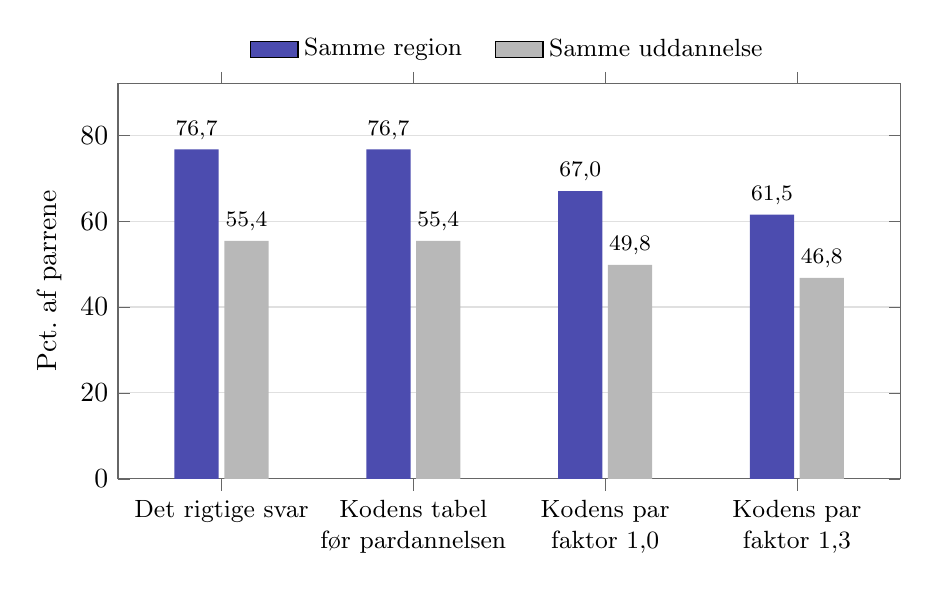
\begin{tikzpicture}
\begin{axis}[
  ybar, area legend, bar width=16pt, width=0.95\textwidth, height=6.6cm,
  ymin=0, ymax=92, enlarge x limits=0.18,
  ylabel={Pct. af parrene},
  symbolic x coords={a,b,c,d}, xtick=data,
  xticklabels={{Det rigtige svar},{Kodens tabel\\før pardannelsen},{Kodens par\\faktor 1,0},{Kodens par\\faktor 1,3}},
  x tick label style={align=center, font=\small},
  ymajorgrids, grid style={black!12}, axis line style={black!60}, tick style={black!60},
  nodes near coords,
  nodes near coords style={font=\footnotesize, /pgf/number format/.cd, fixed, fixed zerofill, precision=1, use comma},
  legend style={at={(0.5,1.03)}, anchor=south, legend columns=2, draw=none, font=\small, /tikz/every even column/.append style={column sep=1em}},
]
\addplot[fill=blue!55!black!70, draw=none] coordinates {(a,76.7) (b,76.7) (c,67.0) (d,61.5)};
\addplot[fill=black!28, draw=none] coordinates {(a,55.4) (b,55.4) (c,49.8) (d,46.8)};
\legend{Samme region, Samme uddannelse}
\end{axis}
\end{tikzpicture}
\caption{Andel af parrene, hvor manden og kvinden bor i samme region og har samme uddannelse. Kodens
tabel før pardannelsen er genberegnet i testen og har de samme andele for begge faktorer. Faktoren er
modellens opskalering af puljen; 1,0 betyder ingen opskalering.}
\label{fig:sortering}
\end{figure}


\section{Baggrund: hvad SBAM gør}\label{sec:sbam}

\subsection{Opgaven}

En mikrosimulationsmodel skal hvert år danne nye par. Det sker i to trin. Først udvælges de enlige,
der skal finde en partner i året; de udgør \emph{puljen}. Derefter skal mændene og kvinderne i puljen
sættes sammen to og to. Det andet trin kaldes matching, og det er det, notatet handler om.

Matchingen skal gengive, at par ikke dannes tilfældigt. Partnere ligner typisk hinanden i alder og
uddannelse og bor i nærheden af hinanden. Mønsteret i, hvem der danner par med hvem, kaldes i
notatet \emph{sorteringen}.

Personerne inddeles i \emph{typer}. En type er en kombination af kendetegn, for eksempel en
30-årig mand med erhvervsuddannelse bosat i Østjylland. Sorteringen kan så skrives som en
\emph{partabel} med en række for hver type mand og en søjle for hver type kvinde. Hvert felt i
tabellen, en \emph{celle}, indeholder antallet af par af netop den kombination.

\subsection{Algoritmen i tre trin}

SBAM (Sparse Biproportionate Adjustment Matching) bygger på en partabel fra historiske data.

\begin{enumerate}
\item \textbf{Historisk tabel.} De par, der blev dannet i en årrække, tælles op i en partabel $X^0$.
Tabellen viser det historiske mønster, men passer ikke til årets pulje, som har en anden størrelse og
sammensætning.

\item \textbf{Tilpasning til puljen (RAS).} Tabellen tilpasses, så summen af hver række er lig
antallet af mænd af den type i puljen, og summen af hver søjle er lig antallet af kvinder. Det gøres
ved skiftevis at gange hver række og hver søjle med en faktor, indtil summerne passer. Metoden kaldes
RAS eller biproportional tilpasning. Én skalering af alle rækker og én af alle søjler kaldes her et
\emph{gennemløb}. Tilpasningen bevarer mønsteret i den historiske tabel så godt, som puljen
tillader.

\item \textbf{Pardannelse.} For hver celle i den tilpassede tabel udtages så mange par, som cellen
angiver, tilfældigt blandt puljens mænd og kvinder af de to typer. Cellerne indeholder normalt ikke
hele tal, så der skal afrundes. Det kan gøres ved lodtrækning: en celle med værdien 2,3 giver to par
og med sandsynlighed 0,3 et tredje.
\end{enumerate}

Et eksempel med to typer af hvert køn viser trin 2. Historisk blev der dannet 200 par, flest mellem
ens typer. Årets pulje har 60 mænd af type 1 og 40 af type 2 og 50 kvinder af hver type:

\begin{center}
\begin{tabular}{@{}lrrcrrr@{}}
\toprule
 & \multicolumn{2}{c}{Historisk tabel $X^0$} & & \multicolumn{3}{c}{Tilpasset til puljen} \\
\cmidrule(lr){2-3}\cmidrule(l){5-7}
 & Kvinde 1 & Kvinde 2 & & Kvinde 1 & Kvinde 2 & Mænd i puljen \\
\midrule
Mand 1 & 80 & 20 & & 44,1 & 15,9 & 60 \\
Mand 2 & 20 & 80 & & 5,9 & 34,1 & 40 \\
\midrule
Kvinder i puljen & & & & 50 & 50 & \\
\bottomrule
\end{tabular}
\end{center}

Den tilpassede tabel bruger alle i puljen, og par mellem ens typer er stadig langt de hyppigste. I
trin 3 giver cellen øverst til venstre 44 par og med sandsynlighed 0,1 et par mere.

\subsection{Det særlige ved koden i SMILE}

Fire forhold i \kode{Matching.cs} har betydning for testen:

\begin{itemize}
\item \textbf{Mange typer.} En type er en kombination af køn, alder (15--65 år), uddannelse
(5 niveauer), bopæl (11 landsdele eller 98 kommuner) og herkomst (5 grupper). Det giver 28.050 typer
med landsdele og 249.900 med kommuner.

\item \textbf{Mænd og kvinder står i samme tabel.} Koden har én liste af typer, hvor kønnet indgår i
typen. Et par tælles derfor i to celler, der er hinandens spejlbilleder. Før pardannelsen lægges de
to celler sammen, så en celles værdi i koden er to gange det antal par, cellen skal give.

\item \textbf{Puljen er større end nødvendigt.} Modellen ganger sandsynligheden for at komme i puljen
med en faktor, \kode{MatchingScaleUp}, som er mellem 1,05 og 1,3 afhængigt af kommune. Koden danner
derefter kun så mange par, som svarer til puljens størrelse divideret med faktoren, og standser. Med
faktor 1,3 forbliver omkring 23 pct. af puljen altså uden partner. Overskuddet skal sikre, at
antallet af par kan nås.

\item \textbf{Pardannelsen sker i flere omgange.} Koden går cellerne igennem op til 1000 gange og
tager højst ét par fra en celles heltalsdel pr. gang. Det er beskrevet nærmere i
afsnit~\ref{sec:fortolkning}.
\end{itemize}

\subsection{Begreber i notatet}

\begin{center}
\begin{tabular}{@{}lp{11.3cm}@{}}
\toprule
Begreb & Betydning \\
\midrule
Type & En kombination af kendetegn for en person: alder, uddannelse, bopæl og i SMILE også herkomst. \\
Pulje & De enlige, der i et år er udvalgt til at danne par. \\
Partabel & Antallet af par for hver kombination af mandens og kvindens type. \\
Celle & Ét felt i partabellen. \\
Sortering & Mønsteret i, hvem der danner par med hvem, altså parrenes fordeling på celler. \\
RAS & Skiftevis skalering af rækker og søjler, til tabellens summer passer med puljen. \\
Gennemløb & I RAS én skalering af alle rækker og alle søjler. I pardannelsen én tur gennem alle celler. \\
Faktor & Modellens opskalering af puljen, \kode{MatchingScaleUp}. Faktor 1,0 er ingen opskalering. \\
Seed & Startværdi for de tilfældige tal. Samme seed giver samme kørsel. \\
\bottomrule
\end{tabular}
\end{center}


\section{Testens opstilling}\label{sec:opstilling}

\subsection{Idéen}

På virkelige data kan man ikke afgøre, om en matching-algoritme rammer rigtigt, fordi det sande
mønster ikke kendes. Testen bruger derfor et kunstigt marked, hvor det gør. Den har fem trin:

\begin{enumerate}
\item Der opstilles et marked med enlige mænd og kvinder og en \emph{sand partabel} $\mu$, som
angiver, hvor mange par der i gennemsnit dannes på et år i hver celle.
\item Ud fra den sande tabel trækkes fem års »registerdata«: de par, der tilfældigvis blev dannet i
hvert af årene. Det er de historiske data, koden får.
\item Der udvælges en pulje af enlige, som skal danne par.
\item \kode{Matching.cs} læser de historiske data og danner par af puljen.
\item De dannede par sammenlignes med den sande tabel og med det, en korrekt SBAM ville give.
\end{enumerate}

\subsection{Det kunstige marked}

Markedet er konstrueret til testen. Alt, hvad der er nødvendigt for at forstå testen, står her.
Bilag~\ref{app:parametre} beskriver markedet fuldt ud med alle parameterværdier og
beregningsmetoden, så det kan genskabes.

\textbf{Typer og befolkning.} En type er en kombination af alder (20--54 år i etårige trin),
uddannelse (3 niveauer) og region (4 regioner). Det giver 420 typer for hvert køn og
$420\times420=176.400$ celler i partabellen. Der er 299.997 enlige mænd og 300.003 enlige kvinder.
Der er flest unge, kvinderne er i gennemsnit bedre uddannede end mændene, og region~1 er den største
og bedst uddannede.

\textbf{Den sande partabel.} Tabellen er beregnet med Choo og Siows (2006) model af
ægteskabsmarkedet. I modellen afhænger antallet af par mellem mænd af type $x$ og kvinder af type $y$
af to ting: hvor mange enlige der er af de to typer, og hvor stor en gevinst $\Phi_{xy}$ de to har
ved at danne par frem for at forblive enlige:
\[
\mu_{xy}=\sqrt{\mu_{x0}\,\mu_{0y}}\;\exp(\Phi_{xy}/2) .
\]
Her er $\mu_{x0}$ og $\mu_{0y}$ antallet af mænd og kvinder af de to typer, der forbliver enlige.
Alle enlige danner enten par eller forbliver enlige, så
$\mu_{x0}+\sum_y\mu_{xy}=M^A_x$ og $\mu_{0y}+\sum_x\mu_{xy}=M^B_y$, hvor $M^A_x$ og $M^B_y$ er antallet
af enlige mænd og kvinder af hver type. Ligningerne har præcis én løsning for en given befolkning
(Decker m.fl., 2013). Den er fundet med iterationsmetoden hos Galichon og Salanié (2022), som er
beskrevet i bilag~\ref{app:parametre}.

Gevinsten er valgt, så mønsteret får de træk, man kender fra virkelige par:
\[
\frac{\Phi_{xy}}{2}=\kappa+h_A(a_x)+h_B(a_y)-\frac{(a_x-a_y-2)^2}{2\,\tau(\bar a_{xy})^2}
+\rho^E_{e_xe_y}+\rho^R_{r_xr_y},
\]
hvor $a$, $e$ og $r$ er alder, uddannelse og region. Leddene betyder:

\begin{itemize}
\item $h_A$ og $h_B$: gevinsten ved at danne par falder med alderen for begge køn, så unge danner
oftere par end ældre.
\item Det kvadratiske led: den foretrukne aldersforskel er, at manden er to år ældre. Tolerancen
$\tau$ for afvigelser vokser med parrets gennemsnitsalder $\bar a_{xy}$ fra 2 til 6 år.
\item $\rho^E$: par med samme uddannelse har en ekstra gevinst, og par med laveste og højeste
uddannelse har et fradrag.
\item $\rho^R$: par på tværs af regioner har et stort fradrag, dog mindre for de to naboregioner 1
og 2.
\item $\kappa$: en konstant, der er sat, så 12 pct. af de enlige mænd finder en partner på et år.
\end{itemize}

Tabel~\ref{tab:marked} viser det marked, der kommer ud af det. Tallene skal ikke ligne et bestemt
land, men størrelsesordenerne er realistiske. Andelen af enlige af en type, der danner par på et år,
kaldes typens \emph{matchrate}.

\begin{table}[ht]
\centering
\caption{Det kunstige marked. Et ekstremt par har en aldersforskel, der ligger mere end 10 år fra den
typiske forskel på 2 år.}
\label{tab:marked}
\begin{tabular}{@{}lr@{}}
\toprule
Enlige mænd & 299.997 \\
Enlige kvinder & 300.003 \\
Nye par pr. år & 36.000 \\
Aldersforskel, gennemsnit (mandens alder minus kvindens, år) & 1,88 \\
Aldersforskel, standardafvigelse (år) & 3,28 \\
Par med samme uddannelse (pct.) & 55,4 \\
Par fra samme region (pct.) & 76,7 \\
Ekstreme par (pct.) & 0,53 \\
Matchrate for mænd på 25 år (pct.) & 17,55 \\
Matchrate for mænd på 50 år (pct.) & 5,80 \\
\bottomrule
\end{tabular}
\end{table}

\textbf{Hvorfor markedet er en rimelig prøve for SBAM.} I Choo og Siows model har den sande tabel
formen $\mu_{xy}=\alpha_x\beta_yK_{xy}$, hvor $K=\exp(\Phi/2)$ ligger fast, og $\alpha$ og $\beta$
afhænger af befolkningen. Den sande tabel for en anden befolkning er derfor en biproportional
tilpasning af den sande tabel for den første. Det er netop den antagelse, SBAM bygger på. En korrekt
SBAM skal altså kunne gengive sorteringen på dette marked, bortset fra den støj, der er i de
historiske data, og den, der kommer fra afrunding. Afviger koden mere end det, er det kodens fejl og
ikke metodens.

\subsection{Historiske data}

Virkelige registerdata er ikke den sande tabel, men ét tilfældigt udfald af den. Det efterlignes ved
at trække antallet af par i hver celle fra en Poisson-fordeling med middelværdi $\mu_{xy}$,
uafhængigt for hver celle og hvert år. Der trækkes fem år, og summen kaldes $X^0$. Den indeholder
180.627 par fordelt på 36.454 af de 176.400 celler; resten er tomme.

Parrene skrives til en tekstfil i det format, \kode{Matching.cs} læser, med én linje for hver person
i hvert par.

\subsection{Puljen}

I SMILE er det andre dele af modellen, der bestemmer, hvem der kommer i puljen. I testen efterlignes
det sådan: hver enlig kommer i puljen med en sandsynlighed, der er lig den andel af hans eller hendes
type, som dannede par pr. år i de historiske data. Mænd og kvinder trækkes uafhængigt, så der kommer
ikke præcis lige mange af hvert køn. Den største side skæres derfor tilfældigt ned til den mindste.
Antallet af mænd og kvinder af hver type i puljen kaldes $n^A_x$ og $n^B_y$.

Med en faktor $s$ over 1 ganges sandsynligheden for at komme i puljen med $s$, som modellen gør.
Puljen bliver så $s$ gange større, og koden danner kun par af cirka $1/s$ af den.

\subsection{Sådan er markedet lagt ind i SMILEs typer}\label{sec:indlejring}

Koden regner med SMILEs 28.050 typer, mens markedet har 840 (420 for hvert køn). Markedets typer er
derfor oversat til SMILEs:

\begin{center}
\begin{tabular}{@{}ll@{}}
\toprule
Markedet & SMILE \\
\midrule
Alder 20--54 & Samme alder \\
Uddannelse 1, 2, 3 & Grundskole, erhvervsfaglig og lang videregående uddannelse \\
Region 1, 2, 3, 4 & Landsdelene København by, Københavns omegn, Fyn og Østjylland \\
 & Kommunerne København, Gentofte, Odense og Aarhus \\
Herkomst & Dansk oprindelse for alle \\
År for de historiske data & 2008--2012, som er de år, koden vælger ud \\
\bottomrule
\end{tabular}
\end{center}

To valg i oversættelsen har betydning for, hvad testen måler:

\begin{itemize}
\item \textbf{Alderen i datafilen er sat ét år ned.} Koden lægger 1 til alderen, når den læser de
historiske data, fordi modellens data måler alderen ved årets begyndelse, mens matchingen sker ved
årets slutning. Datafilen er lavet, så de historiske par og puljen ender i samme typer.
\item \textbf{Alle typer i puljen findes i de historiske data.} En type uden historiske par har
matchrate 0 og kommer aldrig i puljen.
\end{itemize}

\subsection{Hvad kodens par sammenlignes med}

De par, koden danner, tælles op i en partabel $T$. Den sammenlignes med fire andre tabeller:

\begin{description}[leftmargin=1.5em, style=nextline]
\item[Sand model] Den sande tabel $\mu$. Det er det rigtige svar.
\item[Sand model, ét træk] Ét tilfældigt udfald af den sande tabel, trukket på samme måde som et år
af de historiske data. Selv en perfekt algoritme rammer ikke $\mu$ præcist i en enkelt kørsel, fordi
antallet af par i en celle er tilfældigt. Denne tabel viser, hvor stor en afvigelse det giver.
\item[Reference-SBAM] SBAM udført korrekt: den historiske tabel $X^0$ tilpasset til puljen med RAS,
indtil summerne passer. Det er den tilpassede tabel selv, altså før afrunding til hele par.
\item[Kodens RAS-tabel] Den tabel, koden når frem til, når dens RAS stopper efter to gennemløb
(afsnit~\ref{sec:ras}). Tabellen er genberegnet i testprogrammet efter samme fremgangsmåde som
koden; den er ikke aflæst inde fra koden.
\end{description}

Sammenligningen bruger to slags mål. Det første er enkle nøgletal for parrene: aldersforskellen og
dens spredning, andelen af ekstreme par og andelen med samme uddannelse og samme region.

Det andet er et samlet mål for, hvor forskelligt to tabeller fordeler parrene.
Dissimilaritetsindekset (Duncan og Duncan, 1955) er
\[
D=50\sum_{g,h}\left|\frac{T_{gh}}{T_{\cdot\cdot}}-\frac{\mu_{gh}}{\mu_{\cdot\cdot}}\right| ,
\]
hvor $T_{gh}/T_{\cdot\cdot}$ er den andel af parrene i tabellen $T$, der ligger i celle $(g,h)$, og
$\mu_{gh}/\mu_{\cdot\cdot}$ er den tilsvarende andel i den tabel, der sammenlignes med. $D$ er den
andel af parrene i pct., der skulle flyttes til en anden celle, for at de to fordelinger blev ens. Er
$D=10$, ligger hvert tiende par altså forkert. Indekset afhænger ikke af, hvor mange par der er.

Indekset beregnes på fire grupperinger af typerne: alder i etårige trin ($D_{\text{alder}}$),
uddannelse ($D_{\text{udd}}$), region ($D_{\text{reg}}$) og en samlet gruppering efter femårs
aldersgrupper, uddannelse og region ($D_{\text{samlet}}$). Jo finere gruppering, desto mere fylder
tilfældighederne i indekset. Derfor skal kodens $D$ altid holdes op mod rækken »ét træk«.


\section{Resultater}\label{sec:resultater}

\subsection{De tre kørsler}

Der er lavet tre kørsler med de samme historiske data og samme seed
(tabel~\ref{tab:koersler}): én uden opskalering, én med faktor 1,3 og én uden opskalering, hvor koden
inddeler efter kommuner i stedet for landsdele.

\begin{table}[ht]
\centering
\caption{Antal par i de tre kørsler. Målet er det antal par, koden selv beregner, at den skal danne.
De to nederste linjer er kodens egne tællere.}
\label{tab:koersler}
\begin{tabular}{@{}lrrr@{}}
\toprule
 & Faktor 1,0 & Faktor 1,3 & Faktor 1,0 \\
 & landsdele & landsdele & kommuner \\
\midrule
Personer i puljen & 72.666 & 94.366 & 72.666 \\
Mål for antal par & 36.332 & 36.293 & 36.332 \\
Dannede par & 36.132 & 36.293 & 36.132 \\
\quad i pct. af målet & 99,45 & 100,00 & 99,45 \\
Personer uden partner & 402 & 21.780 & 402 \\
\quad i pct. af puljen & 0,55 & 23,08 & 0,55 \\
Gennemløb i RAS & 2 & 2 & 2 \\
Tid i matchingen (sek.) & 1,0--1,4 & 0,1 & 1,1--1,2 \\
\midrule
Forsøg, der gav et par (\kode{succes}) & 36.132 & 36.293 & 36.132 \\
Forsøg, der manglede en person (\kode{udeladt}) & 22.882 & 5.743 & 22.882 \\
\bottomrule
\end{tabular}
\end{table}

Antallet af par rammes i alle tre kørsler. Testprogrammet kontrollerer desuden fire ting, som alle er
i orden: ingen husholdning indgår i mere end ét par, alle matchede var i puljen, ingen par har samme
køn, og antallet af par overstiger ikke målet.

Kørslen med kommuner danner præcis de samme par som kørslen med landsdele. Det er forventet, fordi
markedets fire regioner svarer en-til-en til fire kommuner. Kørslen viser derfor kun, at koden også
kører med kommuneopdelte typer.

\subsection{RAS-tilpasningen stopper for tidligt}\label{sec:ras}

Koden melder i alle tre kørsler, at RAS stoppede i andet gennemløb. Årsagen er en fejl i den test,
der skal afgøre, om tilpasningen er færdig (\kode{RASMatrix.cs}, linje 521--527):

{\small
\begin{verbatim}
        err = (r_ssq + c_ssq) / n;
        //if (ConsoleMessage) Console.WriteLine("--> {0}", err);
        double err0 = err;
        if (err < errOK) break;
        if (itt > ittMax) break;
        if (itt > 0 && err - err0 < 0.00001) break;
        itt++;
\end{verbatim}
}

\kode{err} måler, hvor langt tabellens summer er fra puljen. Næstsidste linje skal standse løkken,
når fejlen ikke længere bliver mindre fra et gennemløb til det næste. Men \kode{err0}, som skulle
huske fejlen fra forrige gennemløb, sættes lig den nye fejl lige inden sammenligningen. Forskellen er
derfor altid 0, og løkken standser i andet gennemløb, uanset hvor stor fejlen er.

Tilpasningen er ikke færdig på det tidspunkt. Summerne afviger med i alt 2.103 personer ud af 72.666,
målt undervejs i andet gennemløb, og en korrekt RAS skal bruge 61 gennemløb på de samme data.

Konsekvensen for sorteringen er alligevel lille på dette marked. Tabellen efter to gennemløb har
samme andel par med samme uddannelse og region som den færdige og afviger 0,9 pct. fra den, målt med
$D_{\text{samlet}}$ (tabel~\ref{tab:mod_reference}). Det gælder, når puljen ligner den befolkning,
de historiske data kommer fra, som den gør her. Testen siger ikke noget om en pulje, der afviger
mere.

\subsection{Sorteringen uden opskalering}

Tabel~\ref{tab:sortering10} viser sorteringen i kørslen med faktor 1,0. De fire øverste rækker
ligger tæt på hinanden: reference-SBAM og kodens RAS-tabel rammer det rigtige svar omtrent lige så
godt som ét tilfældigt udfald af den sande model. De par, koden danner, afviger derimod tydeligt:

\begin{itemize}
\item Andelen af par fra samme region er 67,0 pct. mod 76,7, og andelen med samme uddannelse er
49,8 pct. mod 55,4.
\item Aldersforskellen spreder mere: standardafvigelsen er 3,62 år mod 3,28, og andelen af ekstreme
par er 0,70 pct. mod 0,53.
\item Samlet ligger 15,7 pct. af parrene forkert ($D_{\text{samlet}}$), mod 5,0 pct. for
reference-SBAM og 8,8 pct. for ét tilfældigt udfald.
\end{itemize}

Den gennemsnitlige aldersforskel er derimod ramt (1,90 år mod 1,88).

\begin{table}[ht]
\centering
\caption{Sortering sammenlignet med den sande model, faktor 1,0. $D$ er den andel af parrene i pct.,
der ligger forkert i forhold til den sande model.}
\label{tab:sortering10}
\small
\begin{tabular}{@{}lrrrrrrrrrr@{}}
\toprule
 & & \multicolumn{2}{c}{Aldersforskel} & Eks- & \multicolumn{2}{c}{Samme} & \multicolumn{4}{c}{$D$ mod den sande model} \\
\cmidrule(lr){3-4}\cmidrule(lr){6-7}\cmidrule(l){8-11}
 & Par & gns. & std. & treme & udd. & reg. & alder & udd. & reg. & samlet \\
\midrule
Sand model & 36.000 & 1,88 & 3,28 & 0,53 & 55,4 & 76,7 & 0,00 & 0,00 & 0,00 & 0,00 \\
Sand model, ét træk & 36.280 & 1,84 & 3,28 & 0,55 & 55,1 & 76,7 & 4,34 & 0,52 & 0,57 & 8,77 \\
Reference-SBAM & 36.333 & 1,97 & 3,28 & 0,53 & 55,4 & 76,7 & 2,85 & 0,70 & 0,48 & 5,03 \\
Kodens RAS-tabel & 36.333 & 1,89 & 3,28 & 0,52 & 55,4 & 76,7 & 2,63 & 0,68 & 0,41 & 4,92 \\
Kodens par & 36.132 & 1,90 & 3,62 & 0,70 & 49,8 & 67,0 & 8,22 & 5,66 & 9,68 & 15,72 \\
\bottomrule
\end{tabular}
\end{table}

Tabel~\ref{tab:mod_reference} sammenligner i stedet med reference-SBAM. Så indgår støjen i de
historiske data ikke i sammenligningen, og kun forskellen mellem koden og en korrekt SBAM er tilbage.
Rækken »ét træk« er ét tilfældigt udfald af referencetabellen og viser, hvor meget tilfældigheder
alene giver. For uddannelse og region ligger kodens par 14--18 gange over det niveau med faktor 1,0.

\begin{table}[ht]
\centering
\caption{Sortering sammenlignet med reference-SBAM. $D$ er den andel af parrene i pct., der ligger
forkert i forhold til reference-SBAM.}
\label{tab:mod_reference}
\begin{tabular}{@{}lrrrr@{}}
\toprule
 & $D_{\text{alder}}$ & $D_{\text{udd}}$ & $D_{\text{reg}}$ & $D_{\text{samlet}}$ \\
\midrule
\multicolumn{5}{@{}l}{\emph{Faktor 1,0}} \\
Reference-SBAM, ét træk (tilfældigheder alene) & 4,23 & 0,31 & 0,70 & 8,88 \\
Kodens RAS-tabel & 0,93 & 0,05 & 0,11 & 0,90 \\
Kodens par & 7,85 & 5,61 & 9,62 & 14,72 \\
\midrule
\multicolumn{5}{@{}l}{\emph{Faktor 1,3}} \\
Reference-SBAM, ét træk (tilfældigheder alene) & 3,78 & 0,69 & 0,47 & 7,82 \\
Kodens RAS-tabel & 0,45 & 0,02 & 0,07 & 0,47 \\
Kodens par & 14,62 & 9,33 & 15,18 & 24,67 \\
\bottomrule
\end{tabular}
\end{table}

\subsection{Sorteringen med opskalering}

Med faktor 1,3 er puljen på 47.183 mænd og 47.183 kvinder. Koden danner 36.293 par og standser, så
21.780 personer forbliver uden partner. Sorteringen er svagere end uden opskalering
(tabel~\ref{tab:sortering13}): 61,5 pct. af parrene er fra samme region og 46,8 pct. har samme
uddannelse, standardafvigelsen på aldersforskellen er 3,89 år, og 25,4 pct. af parrene ligger
forkert.

\begin{table}[ht]
\centering
\caption{Sortering sammenlignet med den sande model, faktor 1,3. Rækkerne for den sande model er de
samme som i tabel~\ref{tab:sortering10}.}
\label{tab:sortering13}
\small
\begin{tabular}{@{}lrrrrrrrrrr@{}}
\toprule
 & & \multicolumn{2}{c}{Aldersforskel} & Eks- & \multicolumn{2}{c}{Samme} & \multicolumn{4}{c}{$D$ mod den sande model} \\
\cmidrule(lr){3-4}\cmidrule(lr){6-7}\cmidrule(l){8-11}
 & Par & gns. & std. & treme & udd. & reg. & alder & udd. & reg. & samlet \\
\midrule
Reference-SBAM & 47.183 & 1,91 & 3,28 & 0,52 & 55,4 & 76,7 & 2,54 & 0,56 & 0,35 & 4,72 \\
Kodens RAS-tabel & 47.183 & 1,87 & 3,27 & 0,52 & 55,4 & 76,7 & 2,49 & 0,57 & 0,32 & 4,67 \\
Kodens par & 36.293 & 1,89 & 3,89 & 0,85 & 46,8 & 61,5 & 14,73 & 8,96 & 15,23 & 25,35 \\
\bottomrule
\end{tabular}
\end{table}

De, der får en partner, er heller ikke et tilfældigt udsnit af puljen. Fordelingen på de 840 typer
blandt dem, der får en partner, afviger 12,2 pct. fra puljens fordeling, målt med samme indeks. Hvis
de 23 pct. uden partner var valgt tilfældigt, ville afvigelsen efter et groft overslag ligge under
2--3 pct.\footnote{Overslaget er lavet i hånden ud fra antallet af personer og typer og er ikke
beregnet i testen.} Opskaleringen forskyder altså også, hvilke typer der finder en partner. Testen
har ikke opgjort, hvilke typer der får for få.


\section{Hvor opstår tabet af sortering?}\label{sec:fortolkning}

Kodens RAS-tabel har 76,7 pct. par fra samme region, og de par, koden danner ud fra den, har 67,0
pct. Tabet opstår altså i det sidste trin, pardannelsen, og ikke i data, typeinddeling eller RAS.

Den konklusion forudsætter, at testens genberegning af RAS-tabellen svarer til den tabel, koden
faktisk arbejder med. To ting taler for det: summen af kodens tabel er lig puljens størrelse
(72.666), og koden melder ingen typer, den ikke kender.

\subsection{Sådan danner koden par}

Pardannelsen står i \kode{Matching.cs}, linje 494--515. For hver celle \kode{c} gør koden følgende,
hvor \kode{c.Value} som nævnt er to gange det antal par, cellen skal give:

{\small
\begin{verbatim}
                    int n = 1;  // Antal par der skal laves
                    if (c.Value >= 2.0)
                        c.Value -= 2.0;
                    else
                        n = 0;
                    ...
                    if (c.Value < 2.0)
                    {
                        if (Simulation.Random.NextEvent(c.Value / 2.0))
                        {
                            n++;  //n = 1
                            c.Value = 0;
                        }
                    }
\end{verbatim}
}

Med ord: skal cellen give mindst ét helt par, dannes ét par, og cellens værdi sættes tilsvarende ned.
Er resten derefter under ét par, trækkes der lod: med en sandsynlighed lig resten dannes endnu et
par, og cellen nulstilles. Derefter tages \kode{n} personer fra hver af de to typers lister. Er en
af listerne tom, dannes parret ikke, og forsøget tælles som \kode{udeladt}.

Koden går alle celler igennem på den måde, blander dem og begynder forfra, op til 1000 gange. Den
standser, når målet for antal par er nået.

\subsection{Tre egenskaber, der kan forklare skævheden}

\begin{itemize}
\item \textbf{En rest får et nyt lodtræk i hver omgang.} Hvis lodtrækket ikke giver et par, beholder
cellen sin rest og prøver igen næste gang. En celle, der skal give 0,1 par, har dermed givet et par
med sandsynlighed $1-0{,}9^k$ efter $k$ omgange, og det går mod 1. Efter mange omgange er alle celler
i praksis rundet op.
\item \textbf{Store celler giver kun ét par pr. omgang.} En celle, der skal give 20 par, skal bruge
20 omgange. Imens har hver af de små celler haft 20 lodtræk.
\item \textbf{Personerne går til den, der kommer først.} De små celler bruger personer, som de store
celler skulle have haft i senere omgange. Når en liste er tom, går cellens par tabt.
\end{itemize}

På dette marked er der 36.454 celler med data og 36.333 par at danne, altså i gennemsnit ét par pr.
celle. De store celler er de typiske par: samme region, samme uddannelse og en aldersforskel tæt på
to år. De små celler er de sjældne kombinationer. Når de små celler rundes op på de stores
bekostning, flyttes par fra de typiske til de sjældne kombinationer. Det er den retning, tabellerne
viser.

\subsection{Hvad kodens tællere viser}

\begin{itemize}
\item \textbf{Faktor 1,0.} Målet nås ikke helt, så koden kører alle 1000 omgange. Den gør
$36.132+22.882=59.014$ forsøg på at danne et par, selv om tabellen kun indeholder 36.333 par. De
22.882 forsøg mislykkes, fordi en af de to lister er tom. Det er, hvad man vil forvente, hvis
cellerne rundes op.
\item \textbf{Faktor 1,3.} Koden standser, når målet er nået, og matchingen tager 0,1 sekund mod godt
1 sekund. Her afbrydes de store celler, før de har givet alle deres par, mens de små har haft et
lodtræk i hver omgang. Det passer med, at sorteringen er svagere end med faktor 1,0. Antallet af
omgange er ikke målt.
\end{itemize}

Forklaringen er læst ud af koden og passer med tallene. Den er derefter afprøvet i
afsnit~\ref{sec:nymetode}, hvor pardannelsen sker i én omgang: alle cellens hele par på én gang og én
afgørelse om resten. Sorteringen følger derefter RAS-tabellen.


\section{En ændret metode}\label{sec:nymetode}

Dette afsnit afprøver fem ændringer af koden. Det beskriver, hvad der er ændret og hvorfor, og
måler, hvad ændringerne betyder for præcision og hastighed. Ændring 0--3 retter metoden, så parrene
bliver rigtige. Ændring 4 beregner den samme tabel hurtigere og ændrer ikke resultatet. Ændringerne
er lavet i en kopi af koden, \kode{Matching\_test.cs}. \kode{Matching.cs} er uændret. Hver ændring
kan slås til og fra for sig, så dens virkning kan måles alene.

Hovedresultaterne er:

\begin{itemize}
\item \textbf{Præcision.} Med ændringerne rammer koden det rigtige svar. Med faktor 1,3 er 76,7 pct.
af parrene fra samme region og 55,4 pct. har samme uddannelse, præcis som i den sande model. Kun
1,8 pct. af parrene ligger forkert i forhold til en korrekt SBAM, mod 24,8 pct. med
\kode{Matching.cs}.
\item \textbf{Hastighed.} Ændring 0--3 alene gør koden langsommere i det typiske tilfælde. Med faktor
1,3 tager ét kald af matchingen 74 ms mod 44--46 ms med \kode{Matching.cs}. Med ændring 4 falder
tiden til 32 ms. Uden opskalering, hvor \kode{Matching.cs} bruger omkring 810 ms på at finde de
sidste par, tager den ændrede metode 26 ms. I alle de afprøvede puljer tager den 16--36 ms pr. kald
(afsnit~\ref{sec:hurtigras}).
\item \textbf{En fejl mere.} Undervejs viste det sig, at \kode{Matching.cs} kun bruger den historiske
tabel i modellens første år. I de følgende år er sorteringen derfor endnu svagere end i
afsnit~\ref{sec:fortolkning}: 43,7 pct. af parrene er fra samme region.
\end{itemize}

\subsection{Ændringerne og begrundelsen for dem}\label{sec:aendringer}

Ændringerne har numrene 0--4. De samme numre står i koden (\kode{//TEST0} til \kode{//TEST4}) og i
testens udskrifter. Dette afsnit beskriver ændring 0--3, og
afsnit~\ref{sec:nymetode-praecision}--\ref{sec:andrepuljer} måler deres virkning. Ændring 4 er
beskrevet og målt for sig i afsnit~\ref{sec:hurtigras}.

\subsubsection*{Ændring 0: Den historiske tabel bevares fra år til år}

\textbf{Problemet.} Modellen opretter matchingen én gang, når den starter, og kalder den derefter én
gang for hvert år i fremskrivningen. RAS-tilpasningen ændrer tabellens tal, så efter hvert kald
stiller koden tabellen tilbage med \kode{\_ras.Reset()}. Hver celle husker den værdi, den blev
oprettet med, og får den værdi igen (\kode{RASMatrix.cs}, linje 28--36 og 50--56):

{\small
\begin{verbatim}
    public RASMatrixCell(int row, int col, double value)
    {
      ...
      _value0 = value;
    }
    public void Reset()
    {
      Value = _value0;
\end{verbatim}
}

Men \kode{Matching.cs} opretter én celle med værdien 1 for hvert historisk par og lægger først
bagefter ens celler sammen (linje 156 og 285):

{\small
\begin{verbatim}
    lRas.Add(new RASMatrixCell(j[0], j[1], 1));
    ...
    lRas[i].Value += lRas[i - 1].Value;
\end{verbatim}
}

En celle med 200 historiske par er altså oprettet med værdien 1 og har fået værdien 200 ved
sammenlægningen. \kode{Reset()} sætter den tilbage til 1. Efter det første kald har alle celler
værdien 1. Fra modellens andet år ved tabellen kun, \emph{om} en kombination er set i data, ikke
\emph{hvor ofte}. Almindelige og sjældne kombinationer tæller lige meget.

\textbf{Ændringen.} Cellernes værdier gemmes, når tabellen er lagt sammen, og \kode{Reset()}
gendanner dem.

Fejlen kan ikke ses i afsnit~\ref{sec:resultater}, hvor matchingen kun kaldes én gang. Her er den
påvist ved at kalde den uændrede \kode{Matching.cs} to gange efter hinanden. At modellen opretter
matchingen én gang og kalder den hvert år, er læst i \kode{Demographics.cs}; modellen er ikke kørt.

\subsubsection*{Ændring 1: RAS-tilpasningen kører, til summerne passer}

\textbf{Problemet.} RAS-tilpasningen stopper altid i andet gennemløb på grund af fejlen i
afsnit~\ref{sec:ras}.

\textbf{Ændringen.} Fejlen fra forrige gennemløb huskes rigtigt. Tilpasningen stopper, når summernes
samlede afvigelse er under en milliontedel af det, de skal summere til, når afvigelsen ikke længere
falder, eller når
et loft over antallet af gennemløb er nået. Loftet kan vælges. Det er afprøvet med 10 og 200.

\subsubsection*{Ændring 2: Tabellen indeholder netop de par, der skal dannes}

\textbf{Problemet.} \kode{Matching.cs} tilpasser tabellen til hele puljen. Med faktor 1,3 indeholder
tabellen derfor 30 pct. flere par, end der skal dannes, og koden standser midt i tabellen, når
antallet er nået. Hvilke celler der når at give deres par, afhænger af rækkefølgen.

\textbf{Ændringen.} Hver person tæller $1/s$ i de summer, tabellen tilpasses til, hvor $s$ er
faktoren for personens kommune. Tabellen indeholder dermed netop det antal par, der skal dannes, og
alle celler kan give deres par. Opskaleringen bliver en reserve: der er flere personer af hver
type, end tabellen beder om, så en type sjældnere slipper op.

Samtidig skaleres mændenes og kvindernes summer hver for sig til antallet af par. Det er nødvendigt,
fordi RAS kun kan få summerne til at passe, når de er lige store for de to køn, og det er de sjældent
i en pulje. Overskuddet af det ene køn bliver stående uden partner. Ingen type får en større sum end
antallet af personer af typen.

\subsubsection*{Ændring 3: Parrene dannes i ét gennemløb af cellerne}

\textbf{Problemet.} Pardannelsen i \kode{Matching.cs} går cellerne igennem mange gange og runder de
små celler op på de stores bekostning (afsnit~\ref{sec:fortolkning}).

\textbf{Ændringen.} Hver celle behandles én gang. Skal cellen give 2,3 par, dannes de 2 med det
samme, og de 0,3 afgøres én gang for alle. Afgørelsen kan træffes på to måder, som begge er afprøvet:

\begin{itemize}
\item \textbf{Uafhængig lodtrækning.} Cellen får et ekstra par med sandsynlighed 0,3, uafhængigt af
de andre celler. Det er metoden fra afsnit~\ref{sec:sbam}.
\item \textbf{Systematisk udvælgelse.} Cellerne lægges i en fast rækkefølge, og de forventede antal
par lægges sammen hen over cellerne fra et tilfældigt startpunkt mellem 0 og 1. En celle får et par,
hver gang den løbende sum passerer et helt tal.
\end{itemize}

Et eksempel med fire celler og startpunkt 0,5 viser den systematiske udvælgelse:

\begin{center}
\begin{tabular}{@{}lrrrr@{}}
\toprule
Celle & 1 & 2 & 3 & 4 \\
\midrule
Forventet antal par & 0,4 & 0,3 & 0,6 & 0,7 \\
Løbende sum (starter i 0,5) & 0,9 & 1,2 & 1,8 & 2,5 \\
Par & 0 & 1 & 0 & 1 \\
\bottomrule
\end{tabular}
\end{center}

Summen passerer 1 i celle 2 og 2 i celle 4. De fire celler skal tilsammen give 2,0 par og giver 2.
Det gælder generelt: enhver sammenhængende stribe af celler giver det forventede antal par med en
afvigelse på under ét par, og hver celle får i gennemsnit sit forventede antal. Med uafhængig
lodtrækning er afvigelsen tilfældig og vokser med antallet af celler.

Rækkefølgen afgør, hvad den systematiske udvælgelse rammer præcist. Cellerne sorteres efter parrets
kendetegn: herkomst, region, uddannelse, femårs aldersgruppe og alder, hvert sted for både manden og
kvinden. Celler, der ligner hinanden, står dermed ved siden af hinanden. Antallet af par med for
eksempel en bestemt kombination af regioner og uddannelser rammes så med en afvigelse på under ét
par. Til sammenligning er udvælgelsen også afprøvet i den rækkefølge, typerne tilfældigvis har i
koden.

Til sidst tages personerne fra de to typers lister. Cellerne tages i tilfældig rækkefølge, så det
ikke er bestemte celler, der mister par, hvis en type slipper op.

\subsubsection*{Tilvalg: opsamlingsrunder}

Afrundingen sker celle for celle. Tabellens summer passer med puljen, men efter afrundingen kan en
type med 3 personer blive bedt om 4 par. Det fjerde par kan ikke dannes og går tabt, og partneren
bliver stående i puljen. Jo færre personer der er af hver type, desto oftere sker det.

I en opsamlingsrunde gentages RAS-tilpasningen og pardannelsen for de personer, der er tilbage, og
det antal par, der mangler. Der køres højst fem runder. Opsamlingsrunderne hører ikke til ændring
0--3 og er slået fra, medmindre andet er nævnt.

\subsection{Sådan er ændringerne afprøvet}

Markedet og de historiske data er de samme som i afsnit~\ref{sec:opstilling}. Der er fire ting, som
er anderledes end i afsnit~\ref{sec:resultater}:

\begin{itemize}
\item \textbf{Flere puljer.} For hver faktor (1,0, 1,05 og 1,3) trækkes 10 puljer med hver sit seed.
Alle metoder får de samme puljer og samme seed til pardannelsen. Tallene er gennemsnit over
puljerne. Derfor afviger tallene for \kode{Matching.cs} en smule fra
afsnit~\ref{sec:resultater}, som bygger på én pulje.
\item \textbf{Første og senere år.} \kode{Matching.cs} køres to gange på hver pulje. Det første
kald svarer til modellens første år. Det andet kald sker uden at læse data ind igen og svarer til
alle senere år.
\item \textbf{Hastighed.} Tiden i ét kald af matchingen måles i millisekunder (ms), og medianen over
puljerne rapporteres. Tiden omfatter alt, hvad kaldet gør: puljen sorteres i typer, tabellen
tilpasses, og parrene dannes. Indlæsningen af de historiske data sker én gang ved start og er ikke
med.
\item \textbf{Andre puljer.} Ud over standardpuljen afprøves tre puljer, der er sværere
(afsnit~\ref{sec:andrepuljer}).
\end{itemize}

Præcisionen måles som i afsnit~\ref{sec:opstilling} med parrenes nøgletal og med
$D_{\text{samlet}}$ i forhold til reference-SBAM. Dertil kommer to mål:

\begin{itemize}
\item \textbf{Andel af målet.} Antal dannede par i pct. af det antal, koden skal danne.
\item \textbf{Typer mod pulje.} Dissimilaritetsindekset mellem fordelingen på de 840 typer blandt
dem, der får en partner, og fordelingen i hele puljen. Et lille tal betyder, at alle typer får en
partner i omtrent samme omfang.
\end{itemize}

Som kontrol er \kode{Matching\_test.cs} kørt med alle ændringer slået fra. Den danner da præcis de
samme par som \kode{Matching.cs}, par for par, i både første og andet kald og for alle puljer.
Forskellene nedenfor skyldes altså ændringerne og ikke kopieringen af koden.

\subsection{Præcision}\label{sec:nymetode-praecision}

Tabel~\ref{tab:trin} viser virkningen af ændringerne én efter én med faktor 1,3, som er den højeste
af modellens faktorer.

\begin{table}[ht]
\centering
\caption{Præcision trin for trin, faktor 1,3, gennemsnit over 10 puljer. $D_{\text{samlet}}$ er den
andel af parrene i pct., der ligger forkert i forhold til reference-SBAM. Med ændring 0 alene giver
alle år det samme som første år. »Ét træk« er ét tilfældigt udfald af referencetabellen og viser, hvad tilfældigheder alene giver.}
\label{tab:trin}
\small\setlength{\tabcolsep}{4.5pt}
\begin{tabular}{@{}lrrrrrr@{}}
\toprule
 & Andel af & \multicolumn{2}{c}{Samme} & Alders- & & Typer \\
\cmidrule(lr){3-4}
 & målet & udd. & reg. & forsk., std. & $D_{\text{samlet}}$ & mod pulje \\
\midrule
Reference-SBAM (det rigtige svar) & 100,00 & 55,4 & 76,7 & 3,28 & 0,00 & -- \\
Reference-SBAM, ét træk & -- & 55,5 & 76,7 & 3,27 & 8,78 & -- \\
\midrule
\kode{Matching.cs}, første år & 100,00 & 46,8 & 61,5 & 3,89 & 24,79 & 12,23 \\
\kode{Matching.cs}, senere år & 100,00 & 41,4 & 43,7 & 4,54 & 42,36 & 13,41 \\
\midrule
Ændring 0+1 & 100,00 & 46,8 & 61,5 & 3,90 & 24,79 & 12,25 \\
Ændring 0+1+2 & 100,00 & 48,0 & 63,6 & 3,85 & 20,72 & 11,90 \\
0+1+2+3, uafhængig lodtrækning & 99,93 & 55,4 & 76,6 & 3,28 & 5,02 & 1,76 \\
0+1+2+3, systematisk, kodens rækkefølge & 99,98 & 55,4 & 76,6 & 3,27 & 3,28 & 1,24 \\
0+1+2+3, systematisk, sorteret & 99,97 & 55,4 & 76,7 & 3,28 & 1,82 & 1,38 \\
\midrule
\multicolumn{7}{@{}l}{\emph{Som linjen ovenfor, men}} \\
\quad uden ændring 2 & 100,00 & 55,4 & 76,7 & 3,28 & 6,98 & 4,18 \\
\quad uden ændring 1 (2 RAS-gennemløb) & 99,97 & 55,4 & 76,7 & 3,28 & 1,94 & 1,43 \\
\quad med højst 10 RAS-gennemløb & 99,97 & 55,4 & 76,7 & 3,28 & 1,83 & 1,41 \\
\quad med højst 10 RAS-gennemløb og opsamling & 100,00 & 55,4 & 76,7 & 3,28 & 1,84 & 1,41 \\
\bottomrule
\end{tabular}
\end{table}

\begin{itemize}
\item \textbf{Fejlen i \kode{Reset()} har stor virkning på dette marked.} I senere år er kun 43,7
pct. af parrene fra samme region mod 61,5 i første år og 76,7 i den sande model, og 42,4 pct. af
parrene ligger forkert. Hvor stor virkningen er i modellen, afhænger af dens data
(afsnit~\ref{sec:nyforbehold}).
\item \textbf{Ændring 3 giver næsten hele forbedringen.} Når parrene dannes i ét gennemløb, rammer
alle nøgletal den sande model, og $D_{\text{samlet}}$ falder fra 20,7 til 5,0 eller lavere. Det
bekræfter forklaringen i afsnit~\ref{sec:fortolkning}: tabet af sortering opstod i pardannelsen.
\item \textbf{Ændring 2 betyder noget, når puljen er opskaleret.} Uden den ligger 7,0 pct. af
parrene forkert i stedet for 1,8, og de, der får en partner, ligner puljen dårligere (4,2 mod
1,4 pct.). Med faktor 1,0 gør ændringen ingen forskel.
\item \textbf{Ændring 1 kan ikke måles på standardpuljen.} To RAS-gennemløb giver samme nøgletal som
en færdig tilpasning. Det er anderledes, når puljen ikke ligner de historiske data
(afsnit~\ref{sec:andrepuljer}).
\item \textbf{Systematisk udvælgelse er mere præcis end uafhængig lodtrækning.} Begge rammer
nøgletallene, men den systematiske udvælgelse har mindre tilfældig variation: 1,8--3,3 pct. af
parrene ligger forkert mod 5,0. Alle tre tal er lavere end de 8,8 pct., som ét tilfældigt udfald af
referencetabellen giver.
\end{itemize}

Tallet 1,8 for den sorterede udvælgelse er et bedste tilfælde. Sorteringen bruger de samme grupper
som $D_{\text{samlet}}$ (femårs aldersgrupper, uddannelse og region), så netop det mål rammes
særlig godt. Tallet 3,3 for kodens rækkefølge er uden den fordel.

Den afvigelse, der er tilbage, er tilfældig og ikke systematisk. Lægges parrene fra de 10 puljer
sammen i én tabel, falder $D_{\text{samlet}}$ for den ændrede metode fra 1,8 til 0,6 pct., som
tilfældige afvigelser gør, når der bliver flere par. For \kode{Matching.cs} i første år er tallet
næsten uændret, 23,8 pct.

Figur~\ref{fig:nymetode} viser de to vigtigste nøgletal.

\begin{figure}[ht]
\centering
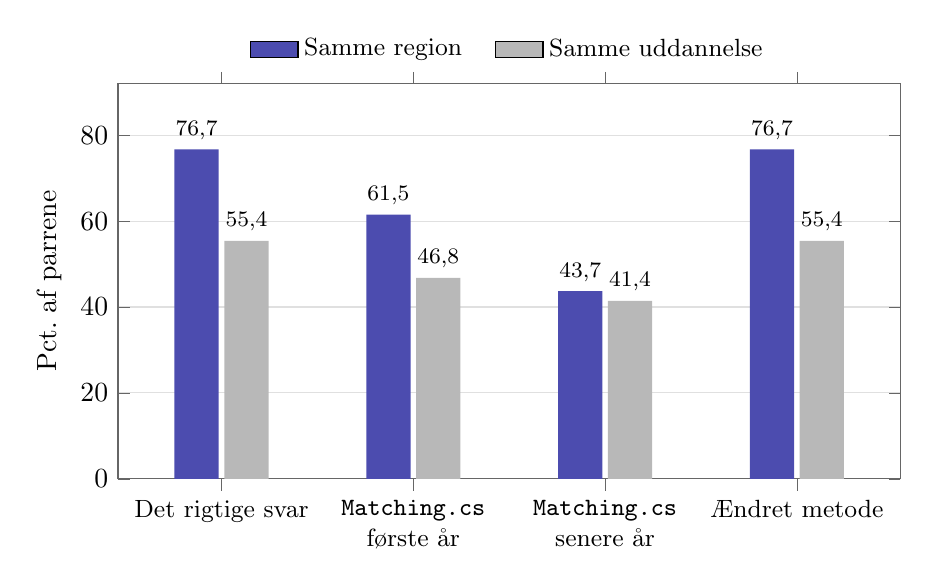
\begin{tikzpicture}
\begin{axis}[
  ybar, area legend, bar width=16pt, width=0.95\textwidth, height=6.6cm,
  ymin=0, ymax=92, enlarge x limits=0.18,
  ylabel={Pct. af parrene},
  symbolic x coords={a,b,c,d}, xtick=data,
  xticklabels={{Det rigtige svar},{\texttt{Matching.cs}\\første år},{\texttt{Matching.cs}\\senere år},{Ændret metode}},
  x tick label style={align=center, font=\small},
  ymajorgrids, grid style={black!12}, axis line style={black!60}, tick style={black!60},
  nodes near coords,
  nodes near coords style={font=\footnotesize, /pgf/number format/.cd, fixed, fixed zerofill, precision=1, use comma},
  legend style={at={(0.5,1.03)}, anchor=south, legend columns=2, draw=none, font=\small, /tikz/every even column/.append style={column sep=1em}},
]
\addplot[fill=blue!55!black!70, draw=none] coordinates {(a,76.7) (b,61.5) (c,43.7) (d,76.7)};
\addplot[fill=black!28, draw=none] coordinates {(a,55.4) (b,46.8) (c,41.4) (d,55.4)};
\legend{Samme region, Samme uddannelse}
\end{axis}
\end{tikzpicture}
\caption{Andel af parrene, hvor manden og kvinden bor i samme region og har samme uddannelse. Faktor
1,3, gennemsnit over 10 puljer. Den ændrede metode er ændring 0--3 med systematisk, sorteret
udvælgelse.}
\label{fig:nymetode}
\end{figure}

\subsection{Hastighed}\label{sec:hastighed}

Tabel~\ref{tab:tid} viser tiden i ét kald af matchingen på standardpuljen med ændring 0--3. Ændring 4
er ikke med her.

\begin{table}[ht]
\centering
\caption{Tid i ét kald af matchingen i ms uden ændring 4, standardpuljen, median over 10 puljer.
Tallene i parentes er den del, der går til RAS-tilpasning og til pardannelse. Resten går til at
sortere puljen i typer og opgøre summerne. \kode{Matching.cs} er uændret og har derfor ingen
opdeling.}
\label{tab:tid}
\small
\begin{tabular}{@{}lrrr@{}}
\toprule
 & Faktor 1,0 & Faktor 1,05 & Faktor 1,3 \\
\midrule
\kode{Matching.cs}, første år & 812 & 50 & 46 \\
\kode{Matching.cs}, senere år & 806 & 41 & 44 \\
\midrule
\multicolumn{4}{@{}l}{\emph{Ændret metode, én runde}} \\
\quad 2 RAS-gennemløb (uden ændring 1) & 30 (12 + 7) & 32 (12 + 8) & 34 (12 + 7) \\
\quad højst 10 RAS-gennemløb & 42 (24 + 7) & 45 (27 + 7) & 47 (25 + 7) \\
\quad RAS, til summerne passer (52--54 gennemløb) & 113 (95 + 7) & 110 (87 + 7) & 112 (90 + 7) \\
\midrule
\multicolumn{4}{@{}l}{\emph{Ændret metode med opsamlingsrunder}} \\
\quad højst 10 RAS-gennemløb pr. runde & 152 (111 + 25) & 89 (50 + 13) & 74 (48 + 12) \\
\quad RAS, til summerne passer & 755 (709 + 26) & 297 (257 + 14) & 207 (179 + 12) \\
\quad Antal runder (med højst 10 gennemløb) & 5,0 & 2,4 & 2,0 \\
\bottomrule
\end{tabular}
\end{table}

\begin{itemize}
\item \textbf{Med opskalering er den ændrede metode lige så hurtig som \kode{Matching.cs} uden
opsamlingsrunder og bruger 1,5--2 gange så lang tid med.} Med faktor 1,05 og 1,3 tager
\kode{Matching.cs} 41--50 ms. Den ændrede metode med højst 10 RAS-gennemløb tager 45--47 ms i én
runde og 74--89 ms med opsamlingsrunder. Forskellen er 28--48 ms pr. kald.
\item \textbf{Uden opskalering er den ændrede metode godt 5 gange hurtigere.} Med faktor 1,0 tager
\kode{Matching.cs} omkring 810 ms, fordi pardannelsen går cellerne igennem mange gange for at finde
de sidste par. Den ændrede metode tager 152 ms med opsamlingsrunder og 42 ms uden. Det samme sker med
faktor 1,05, når der er færre mænd end kvinder i puljen (afsnit~\ref{sec:andrepuljer}).
\item \textbf{Pardannelsen i ét gennemløb tager 7--8 ms uanset faktoren.} Den oprindelige
pardannelse tager 6 ms med faktor 1,3 og 10 ms med faktor 1,05, men omkring 550 ms med faktor 1,0.
De tre tal er målt i varianten med ændring 0+1, som har den oprindelige pardannelse.
\item \textbf{RAS er den største post i den ændrede metode.} Et gennemløb koster omkring 1,5 ms, og
dertil kommer omkring 10 ms pr. tilpasning til det arbejde, der ikke afhænger af antallet af
gennemløb. At køre RAS, til summerne passer, kræver 52--54 gennemløb og koster 60--70 ms mere pr.
runde end et loft på 10. Det giver ingen målelig forbedring på standardpuljen
(tabel~\ref{tab:trin}) og en lille forbedring, når puljen afviger fra de historiske data
(tabel~\ref{tab:ras}). Ændring 4 fjerner det meste af tiden til RAS
(afsnit~\ref{sec:hurtigras}).
\item \textbf{En opsamlingsrunde koster 25--35 ms.} Den består af en ny RAS-tilpasning og en ny
pardannelse. Med faktor 1,3 er der brug for én ekstra runde. Med faktor 1,0 bruges alle fem runder.
\end{itemize}

Tiderne er målt på testens pc. De svinger fra måling til måling, så forskelle på under 10 ms skal
ikke tillægges betydning: fire varianter, der laver næsten samme arbejde, ligger mellem 105 og 112
ms med faktor 1,05 og 1,3.

Tiderne er lavere end i afsnit~\ref{sec:fortolkning}, hvor matchingen tog 0,1 og godt 1 sekund. De
tal er fra et enkelt kald, hvor .NET også skal oversætte koden til maskinkode. Her er medianen over
10 kald brugt, så den tid ikke tæller med.

\subsection{Antal par}

Ændring 3 har en pris. Når en type slipper op, går cellens par tabt. Det sker også i
\kode{Matching.cs}, men den går cellerne igennem igen, til antallet er nået. Med ét gennemløb mangler
de tabte par til sidst. Tabel~\ref{tab:antalpar} viser, hvor stor en del af målet der nås.

\begin{table}[ht]
\centering
\caption{Dannede par i pct. af målet. Den ændrede metode er ændring 0--3 med højst 10
RAS-gennemløb. Den lille pulje og puljen med færre mænd er beskrevet i
afsnit~\ref{sec:andrepuljer}.}
\label{tab:antalpar}
\begin{tabular}{@{}lrrr@{}}
\toprule
 & Faktor 1,0 & Faktor 1,05 & Faktor 1,3 \\
\midrule
\multicolumn{4}{@{}l}{\emph{Standardpulje (36.000 par)}} \\
\kode{Matching.cs}, første år & 99,56 & 100,00 & 100,00 \\
Ændret metode, én runde & 97,83 & 99,36 & 99,97 \\
Ændret metode med opsamlingsrunder & 99,98 & 100,00 & 100,00 \\
\midrule
\multicolumn{4}{@{}l}{\emph{Lille pulje (3.600 par)}} \\
\kode{Matching.cs}, første år & 99,55 & 100,00 & 100,00 \\
Ændret metode, én runde & 88,02 & 90,60 & 96,93 \\
Ændret metode med opsamlingsrunder & 99,87 & 100,00 & 100,00 \\
\midrule
\multicolumn{4}{@{}l}{\emph{10 pct. færre mænd end kvinder}} \\
Højst mulige (alle mænd får en partner) & 94,74 & 99,48 & 100,00 \\
\kode{Matching.cs}, første år & 94,74 & 99,48 & 100,00 \\
Ændret metode, én runde & 93,54 & 98,23 & 99,97 \\
Ændret metode med opsamlingsrunder & 94,73 & 99,47 & 100,00 \\
\bottomrule
\end{tabular}
\end{table}

I standardpuljen mangler 0,03 pct. af parrene med faktor 1,3 og 2,2 pct. med faktor 1,0. I den lille
pulje, hvor der er få personer af hver type, mangler der 3--12 pct. Uden opsamlingsrunder er
ændring 3 derfor ikke brugbar, når puljen er lille i forhold til antallet af typer. Med
opsamlingsrunder nås målet i alle tilfælde, hvor det kan nås, og parrenes sammensætning er
uændret (tabel~\ref{tab:trin} og~\ref{tab:andrepuljer}).

I puljen med færre mænd kan højst 94,74 og 99,48 pct. af målet nås med faktor 1,0 og 1,05, fordi
mændene slipper op. Den forskudte pulje i afsnit~\ref{sec:andrepuljer} giver samme tal som
standardpuljen: 97,5--99,95 pct. i én runde og 99,97--100 pct. med opsamlingsrunder.

\subsection{Andre puljer}\label{sec:andrepuljer}

Standardpuljen ligner de historiske data og har lige mange mænd og kvinder. Tre andre puljer
afprøver, om resultaterne holder, når det ikke er tilfældet:

\begin{itemize}
\item \textbf{Lille pulje.} Puljen er en tiendedel så stor, og der skal dannes 3.600 par. Der er få
personer af hver type: i gennemsnit 11 med faktor 1,3 og 9 med faktor 1,0. 10 puljer pr. faktor.
\item \textbf{Færre mænd.} 10 pct. af puljens mænd er fjernet tilfældigt. 5 puljer pr. faktor.
\item \textbf{Forskudt pulje.} Sandsynligheden for at komme i puljen stiger med alder og uddannelse.
Den er halvt så stor som i standardpuljen for 20-årige og for det laveste uddannelsesniveau og
halvanden gang så stor for 54-årige og for det højeste niveau. Puljen har altså flere ældre og
flere med lang uddannelse end de historiske data. 5 puljer pr. faktor.
\end{itemize}

Målestokken er reference-SBAM, det vil sige en korrekt udført SBAM på den samme pulje. Den sande
model kan ikke bruges i den forskudte pulje, fordi den er beregnet for en befolkning med en anden
sammensætning. Tabel~\ref{tab:andrepuljer} viser resultaterne med faktor 1,3.

\begin{table}[ht]
\centering
\caption{Andre puljer, faktor 1,3. Den ændrede metode er ændring 0--3 med højst 10 RAS-gennemløb og
opsamlingsrunder, uden ændring 4. $D_{\text{samlet}}$ er i forhold til reference-SBAM. Tid er
medianen i ms.}
\label{tab:andrepuljer}
\small
\begin{tabular}{@{}lrrrrrr@{}}
\toprule
 & \multicolumn{2}{c}{Aldersforskel} & \multicolumn{2}{c}{Samme} & & \\
\cmidrule(lr){2-3}\cmidrule(lr){4-5}
 & gns. & std. & udd. & reg. & $D_{\text{samlet}}$ & Tid \\
\midrule
\multicolumn{7}{@{}l}{\emph{Lille pulje}} \\
Reference-SBAM (det rigtige svar) & 1,86 & 3,29 & 55,2 & 76,4 & 0,00 & -- \\
Reference-SBAM, ét træk & 1,85 & 3,31 & 55,0 & 76,2 & 25,84 & -- \\
\kode{Matching.cs}, første år & 1,88 & 3,32 & 53,3 & 75,1 & 24,89 & 26 \\
\kode{Matching.cs}, senere år & 1,84 & 4,32 & 41,8 & 41,8 & 50,29 & 27 \\
Ændret metode & 1,87 & 3,26 & 55,2 & 76,6 & 13,99 & 66 \\
\midrule
\multicolumn{7}{@{}l}{\emph{Færre mænd}} \\
Reference-SBAM (det rigtige svar) & 1,84 & 3,28 & 55,4 & 76,7 & 0,00 & -- \\
Reference-SBAM, ét træk & 1,86 & 3,27 & 55,5 & 77,0 & 9,08 & -- \\
\kode{Matching.cs}, første år & 1,76 & 3,88 & 46,7 & 61,5 & 24,72 & 44 \\
\kode{Matching.cs}, senere år & 1,80 & 4,52 & 41,3 & 43,4 & 42,37 & 46 \\
Ændret metode & 1,85 & 3,28 & 55,4 & 76,7 & 1,93 & 72 \\
\midrule
\multicolumn{7}{@{}l}{\emph{Forskudt pulje}} \\
Reference-SBAM (det rigtige svar) & 1,75 & 3,50 & 58,6 & 76,7 & 0,00 & -- \\
Reference-SBAM, ét træk & 1,75 & 3,50 & 58,7 & 76,9 & 9,68 & -- \\
\kode{Matching.cs}, første år & 1,86 & 4,12 & 50,0 & 62,9 & 23,94 & 44 \\
\kode{Matching.cs}, senere år & 1,84 & 4,73 & 45,0 & 44,6 & 41,51 & 43 \\
Ændret metode & 1,79 & 3,51 & 58,6 & 76,7 & 2,31 & 70 \\
\bottomrule
\end{tabular}
\end{table}

\begin{itemize}
\item \textbf{Den ændrede metode rammer det rigtige svar i alle tre puljer.} Andelene med samme
uddannelse og region afviger højst 0,2 procentpoint fra reference-SBAM, og $D_{\text{samlet}}$
ligger under det, tilfældigheder alene giver.
\item \textbf{I den lille pulje er \kode{Matching.cs} næsten rigtig i første år.} Andelene er 53,3
og 75,1 pct. mod 55,2 og 76,4, og $D_{\text{samlet}}$ er på niveau med tilfældighederne.
Forklaringen er formentlig, at næsten ingen celler skal give mere end ét par i en lille pulje. Så
danner første omgang næsten alle par, og i den har hver celle kun ét lodtræk
(afsnit~\ref{sec:fortolkning}). Antallet af omgange er ikke målt. Skævheden i \kode{Matching.cs} er
altså størst i store puljer. Fejlen i \kode{Reset()} slår derimod fuldt igennem: 41,8 pct. fra samme
region i senere år.
\item \textbf{Med færre mænd bliver aldersforskellen for lille i \kode{Matching.cs}.} Den er 1,76 år
mod 1,84 i reference-SBAM. Den ændrede metode giver 1,85. Uden ændring 2 kan RAS ikke få summerne
til at passe i denne pulje, fordi mændenes og kvindernes summer er forskellige. Tilpasningen
stopper da efter omkring fire gennemløb.
\item \textbf{I den forskudte pulje er aldersforskellen 1,79 år mod 1,75 i reference-SBAM.}
\kode{Matching.cs} giver 1,86. Afvigelsen på 0,04 år skyldes loftet over RAS-gennemløb
(tabel~\ref{tab:ras}).
\end{itemize}

Med faktor 1,0 og 1,05 skal alle mænd i puljen med færre mænd have en partner. Her er der to ting
at bemærke. \kode{Matching.cs} tager 920 og 842 ms mod 157 og 149 ms for den ændrede metode. Og
opsamlingsrunderne flytter den ændrede metode lidt væk fra reference-SBAM: aldersforskellen bliver
1,91--1,92 år mod 1,85--1,86, og standardafvigelsen 3,31--3,32 mod 3,28. De sidste mænd må tage de
kvinder, der er tilbage. \kode{Matching.cs} ligger længere væk med 1,67 år og 3,63--3,64.

Tabel~\ref{tab:ras} viser betydningen af antallet af RAS-gennemløb.

\begin{table}[H]
\centering
\caption{Betydningen af antal RAS-gennemløb. Ændring 0, 2 og 3 i én runde, uden ændring 4, faktor 1,3.
$D_{\text{udd}}$ og $D_{\text{samlet}}$ er i forhold til reference-SBAM. I sidste linje for hver
pulje kører RAS, til summerne passer.}
\label{tab:ras}
\small
\begin{tabular}{@{}lrrrrr@{}}
\toprule
 & RAS- & RAS-tid, & Alders- & & \\
 & gennemløb & ms & forskel & $D_{\text{udd}}$ & $D_{\text{samlet}}$ \\
\midrule
\multicolumn{6}{@{}l}{\emph{Standardpulje (reference-SBAM: 1,85 år)}} \\
Som \kode{Matching.cs} & 2 & 12 & 1,87 & 0,03 & 1,94 \\
Loft på 10 & 10 & 25 & 1,86 & 0,02 & 1,83 \\
Til summerne passer & 54 & 90 & 1,85 & 0,02 & 1,82 \\
\midrule
\multicolumn{6}{@{}l}{\emph{Forskudt pulje (reference-SBAM: 1,75 år)}} \\
Som \kode{Matching.cs} & 2 & 13 & 1,87 & 0,37 & 2,92 \\
Loft på 10 & 10 & 26 & 1,79 & 0,05 & 2,30 \\
Til summerne passer & 67 & 109 & 1,75 & 0,03 & 2,17 \\
\bottomrule
\end{tabular}
\end{table}

I standardpuljen er to gennemløb nok. I den forskudte pulje er de ikke: aldersforskellen bliver
1,87 år, som er tæt på de 1,88 år i den sande model bag de historiske data, og ikke de 1,75, der
passer til puljen. Tabellen når med andre ord ikke at blive tilpasset til puljen. Ti gennemløb fjerner det meste af
afvigelsen og koster 14 ms. Resten kræver 67 gennemløb og 83 ms mere. Loftet er en indstilling og
kan sættes højere, hvis puljerne i modellen afviger mere fra de historiske data end her. Med
ændring 4 koster alle 67 gennemløb 4 ms, og loftet kan undværes (afsnit~\ref{sec:hurtigras}).

Testen er også kørt med kommuneopdelte typer (3 puljer). Det giver samme billede som med landsdele.
Den ændrede metode tager 81 ms mod 53 ms for \kode{Matching.cs} med faktor 1,3 og 174 mod 788 ms
med faktor 1,0.

\subsection{Ændring 4: Den samme tabel beregnes hurtigere}\label{sec:hurtigras}

Afsnit~\ref{sec:hastighed} viste, at RAS-tilpasningen er den største post i den ændrede metode. Med
opsamlingsrunder og højst 10 gennemløb går 48 af 74 ms til RAS med faktor 1,3 og 111 af 152 ms med
faktor 1,0. Ændring 4 beregner den samme tilpassede tabel på en hurtigere måde. Kun regnemåden er
ændret. Ændring 0--3 er de samme som før.

\subsubsection*{Hvor tiden går}

RAS-tilpasningen ligger i \kode{RASMatrix.cs}, som både \kode{Matching.cs} og den ændrede metode
bruger. Tre forhold gør den langsom:

\begin{itemize}
\item \textbf{Hver celle er et selvstændigt objekt.} Cellerne i en række hænger sammen i en kæde,
hvor hver celle peger på den næste, og det samme gælder søjlerne. Programmet må følge kæden fra celle
til celle. Det er langsommere end at læse tal, der ligger på række i hukommelsen.
\item \textbf{Hvert gennemløb går alle celler igennem fire gange.} Rækkerne lægges sammen, rækkernes
celler ganges med en faktor, og derefter sker det samme for søjlerne. Tabellen har 72.908 celler,
fordi hver af de 36.454 celler med data står to gange (afsnit~\ref{sec:sbam}).
\item \textbf{Hvert kald har et fast arbejde.} Efter det sidste gennemløb sorteres alle celler, så de
to spejlbilleder af en celle kan lægges sammen. Bagefter skal alle celler stilles tilbage til
udgangspunktet.
\end{itemize}

\subsubsection*{Ændringen}

Ændringen består af tre greb, 4a--4c, som kan slås til hver for sig.

\textbf{4a: Der regnes på faktorer i stedet for celler.} RAS gør kun én ting: ganger en hel række
eller en hel søjle med et tal. Den tilpassede celle er derfor altid den historiske værdi gange en
faktor for rækken og en faktor for søjlen. I eksemplet i afsnit~\ref{sec:sbam} kan faktorerne være
0,551 for mand 1 og 1,443 for kvinde 2, og cellen bliver $20\cdot 0{,}551\cdot 1{,}443=15{,}9$. Det
er derfor nok at regne på faktorerne, to tal pr. type, og lade de historiske værdier stå urørt. Det
sparer tid fire steder:

\begin{itemize}
\item De historiske værdier ligger i én lang række af tal, række for række, uden kæder.
\item Et gennemløb læser cellerne to gange og skriver ikke i dem.
\item Hvilke celler der er spejlbilleder af hinanden, findes én gang ved start og ikke ved en
sortering i hvert kald.
\item Tabellen skal ikke stilles tilbage efter kaldet. Fejlen bag ændring 0 kan dermed ikke opstå.
\end{itemize}

Gennemløb for gennemløb giver 4a de samme tal som \kode{RASMatrix.cs}, bortset fra afrunding på
sidste decimal.

\textbf{4b: Én faktor pr. type.} I kodens tabel står mænd og kvinder i samme liste af typer, og
hvert par står i to celler, der er spejlbilleder. Rækker og søjler skal passe til de samme summer,
nemlig antallet af personer af hver type. Så kan en type have samme faktor som række og som søjle,
og én faktor pr. type er nok. Typerne tages én ad gangen, og typens faktor sættes, så typens sum
passer, givet de andre typers aktuelle faktorer. Et gennemløb læser cellerne én gang.

Uden par af samme køn er hvert skridt en almindelig RAS-skalering af én række eller én søjle i
tabellen med mænd i rækkerne og kvinder i søjlerne. Kun rækkefølgen er en anden end i 4a.
Resultatet er derfor det samme, når tilpasningen kører, til summerne passer, men ikke gennemløb for
gennemløb. En celle med to personer af samme type kan kun forekomme med par af samme køn. Den giver
en andengradsligning i typens faktor, som løses direkte.

\textbf{4c: Kun typer med personer i puljen.} En type uden personer i puljen har summen 0, og alle
dens celler bliver 0. Der regnes derfor kun på typer med personer i puljen og på celler mellem to
sådanne typer, og kun de celler gives videre til pardannelsen. Grebet virker især i
opsamlingsrunderne, hvor få typer er tilbage. I modellen har tabellen 28.050 typer, og puljen
indeholder næppe dem alle. Dér kan grebet også betyde noget i første runde. Det er ikke målt.

\subsubsection*{Kontrol af, at tabellen er den samme}

\begin{itemize}
\item \textbf{4a danner præcis de samme par.} Den ændrede metode er kørt med og uden 4a på de samme
puljer med samme seed. Parrene er de samme, par for par, i alle 96 kørsler: 30 på standardpuljen,
30 på den lille pulje, 15 med færre mænd, 15 på den forskudte pulje og 6 med kommuneopdelte typer.
\item \textbf{4b og 4c giver ikke de samme par, men samme sammensætning.} Med et loft på 10
gennemløb er tabellen fra 4b en anelse anderledes end tabellen fra 4a. Med 4c får pardannelsen færre
celler og bruger derfor de tilfældige tal anderledes. Nøgletallene er uændrede. På standardpuljen
med faktor 1,3 har 55,4 pct. af parrene samme uddannelse, 76,7 pct. er fra samme region, og
$D_{\text{samlet}}$ er 1,83--1,84 pct. både med og uden ændring 4.
\item \textbf{RAS-delen er kontrolleret for sig.} Regnemåderne er sammenlignet på 20 tilfældige
symmetriske tabeller med 30--59 typer, som også har celler med to af samme type. Alle er kørt, til
summerne passer. Den største relative afvigelse i en celle fra \kode{RASMatrix.cs} er
$3\cdot10^{-13}$ med 4a og $6\cdot10^{-13}$ med 4b.
\end{itemize}

\subsubsection*{Hastighed}

Tabel~\ref{tab:hurtig} viser tiden på standardpuljen, når grebene slås til ét efter ét.

\begin{table}[ht]
\centering
\caption{Tid i ét kald af matchingen i ms med og uden ændring 4, standardpuljen, median over 10
puljer. Alle linjer undtagen \kode{Matching.cs} har ændring 0--3 med systematisk, sorteret
udvælgelse. Tallene i parentes er den del, der går til RAS-tilpasning og til pardannelse.}
\label{tab:hurtig}
\small
\begin{tabular}{@{}lrrr@{}}
\toprule
 & Faktor 1,0 & Faktor 1,05 & Faktor 1,3 \\
\midrule
\kode{Matching.cs}, første år & 812 & 50 & 46 \\
\kode{Matching.cs}, senere år & 806 & 41 & 44 \\
\midrule
\multicolumn{4}{@{}l}{\emph{Højst 10 RAS-gennemløb pr. runde, med opsamlingsrunder}} \\
\quad uden ændring 4 & 152 (111,0 + 24,9) & 89 (50,2 + 13,1) & 74 (48,3 + 12,2) \\
\quad med 4a & 38 (6,4 + 20,4) & 25 (3,6 + 10,8) & 26 (2,5 + 10,6) \\
\quad med 4a og 4b & 36 (4,6 + 21,6) & 24 (2,0 + 10,7) & 25 (1,7 + 11,7) \\
\quad med 4a, 4b og 4c & 22 (2,1 + 8,1) & 24 (2,5 + 9,8) & 24 (2,1 + 10,8) \\
\midrule
\multicolumn{4}{@{}l}{\emph{RAS, til summerne passer, med opsamlingsrunder}} \\
\quad uden ændring 4 & 755 (708,7 + 26,3) & 297 (256,7 + 13,9) & 207 (178,5 + 11,9) \\
\quad med 4a, 4b og 4c & 26 (5,7 + 8,6) & 31 (10,0 + 11,4) & 32 (8,1 + 10,5) \\
\midrule
\multicolumn{4}{@{}l}{\emph{Højst 10 RAS-gennemløb, én runde}} \\
\quad uden ændring 4 & 42 (23,7 + 7,1) & 45 (27,0 + 7,1) & 47 (25,0 + 7,1) \\
\quad med 4a, 4b og 4c & 17 (1,1 + 7,1) & 17 (1,1 + 6,6) & 21 (1,1 + 7,8) \\
\midrule
\multicolumn{4}{@{}l}{\emph{RAS, til summerne passer (52--55 gennemløb), én runde}} \\
\quad uden ændring 4 & 113 (95,4 + 7,3) & 110 (86,7 + 7,2) & 112 (89,9 + 7,3) \\
\quad med 4a, 4b og 4c & 21 (3,3 + 7,2) & 21 (3,4 + 6,7) & 22 (3,4 + 7,0) \\
\bottomrule
\end{tabular}
\end{table}

\begin{itemize}
\item \textbf{RAS-tiden falder til en tyvendedel eller mindre.} Med højst 10 gennemløb pr. runde
falder den fra 48--111 ms til 2,1--2,5 ms. Når RAS kører, til summerne passer, falder den fra
179--709 ms til 6--10 ms.
\item \textbf{4a giver næsten hele gevinsten.} RAS-tiden falder fra 111 til 6,4 ms med faktor 1,0 og
fra 48 til 2,5 ms med faktor 1,3. 4b fjerner mellem en fjerdedel og knap halvdelen af det, der er
tilbage.
\item \textbf{4c virker, når der er mange opsamlingsrunder.} Med faktor 1,0 og fem runder falder
RAS-tiden fra 4,6 til 2,1 ms og pardannelsen fra 22 til 8 ms, fordi pardannelsen i de sidste runder
kun får de få celler, der er tilbage. Med to runder er der ingen målelig forskel.
\item \textbf{Et gennemløb koster 0,05 ms mod 1,5 ms før.} I én runde koster 10 gennemløb 1,1 ms og
52--55 gennemløb 3,3--3,4 ms. Det faste arbejde pr. tilpasning koster dermed omkring 0,6 ms mod
omkring 10 ms før.
\item \textbf{Loftet på 10 gennemløb er overflødigt.} At køre RAS, til summerne passer, koster 4--8 ms
mere pr. kald end et loft på 10: 26, 31 og 32 ms mod 22, 24 og 24. Uden ændring 4 koster det
133--603 ms mere.
\item \textbf{Den ændrede metode er nu mindst lige så hurtig som \kode{Matching.cs} med opskalering
og omkring 30 gange hurtigere uden.} Med RAS, til summerne passer, og opsamlingsrunder tager den
26--32 ms. \kode{Matching.cs} tager 41--50 ms med opskalering og omkring 810 ms uden.
\item \textbf{RAS er ikke længere den største post.} Af de 32 ms med faktor 1,3 går 8 til RAS og 11
til pardannelsen. De sidste omkring 13 ms går til at sortere puljen i typer og opgøre summerne. Den
del er ikke ændret.
\end{itemize}

Som i afsnit~\ref{sec:hastighed} svinger de samlede tider nogle ms fra måling til måling.

\subsubsection*{Alle puljer}

Når RAS er billig, kan den køre, til summerne passer, i alle runder.
Tabel~\ref{tab:hurtigpuljer} sammenligner den metode med metoden fra tabel~\ref{tab:andrepuljer},
som har et loft på 10 gennemløb og ikke bruger ændring 4.

\begin{table}[H]
\centering
\caption{Den ændrede metode med og uden ændring 4, faktor 1,3. Begge har ændring 0--3 og
opsamlingsrunder. $D_{\text{samlet}}$ er i forhold til reference-SBAM. Tid er medianen i ms.}
\label{tab:hurtigpuljer}
\small
\begin{tabular}{@{}lrrrrrr@{}}
\toprule
 & \multicolumn{2}{c}{Aldersforskel} & \multicolumn{2}{c}{Samme} & & \\
\cmidrule(lr){2-3}\cmidrule(lr){4-5}
 & gns. & std. & udd. & reg. & $D_{\text{samlet}}$ & Tid \\
\midrule
\multicolumn{7}{@{}l}{\emph{Standardpulje}} \\
Reference-SBAM (det rigtige svar) & 1,85 & 3,28 & 55,4 & 76,7 & 0,00 & -- \\
Loft på 10 gennemløb, uden ændring 4 & 1,86 & 3,28 & 55,4 & 76,7 & 1,84 & 74 \\
Til summerne passer, med ændring 4 & 1,85 & 3,28 & 55,4 & 76,7 & 1,83 & 32 \\
\midrule
\multicolumn{7}{@{}l}{\emph{Lille pulje}} \\
Reference-SBAM (det rigtige svar) & 1,86 & 3,29 & 55,2 & 76,4 & 0,00 & -- \\
Loft på 10 gennemløb, uden ændring 4 & 1,87 & 3,26 & 55,2 & 76,6 & 13,99 & 66 \\
Til summerne passer, med ændring 4 & 1,87 & 3,25 & 55,2 & 76,6 & 13,78 & 19 \\
\midrule
\multicolumn{7}{@{}l}{\emph{Færre mænd}} \\
Reference-SBAM (det rigtige svar) & 1,84 & 3,28 & 55,4 & 76,7 & 0,00 & -- \\
Loft på 10 gennemløb, uden ændring 4 & 1,85 & 3,28 & 55,4 & 76,7 & 1,93 & 72 \\
Til summerne passer, med ændring 4 & 1,84 & 3,28 & 55,4 & 76,7 & 1,92 & 31 \\
\midrule
\multicolumn{7}{@{}l}{\emph{Forskudt pulje}} \\
Reference-SBAM (det rigtige svar) & 1,75 & 3,50 & 58,6 & 76,7 & 0,00 & -- \\
Loft på 10 gennemløb, uden ændring 4 & 1,79 & 3,51 & 58,6 & 76,7 & 2,31 & 70 \\
Til summerne passer, med ændring 4 & 1,75 & 3,50 & 58,6 & 76,7 & 2,18 & 30 \\
\bottomrule
\end{tabular}
\end{table}

Tabel~\ref{tab:hurtigtid} viser tiden for alle faktorer.

\begin{table}[H]
\centering
\caption{Tid i ét kald af matchingen i ms, median over puljerne. »Ændret« er ændring 0--4 med RAS,
til summerne passer, og opsamlingsrunder. \kode{Matching.cs} er første år. Kommuneopdelte typer er
ikke kørt med faktor 1,05.}
\label{tab:hurtigtid}
\small
\begin{tabular}{@{}lrrrrrr@{}}
\toprule
 & \multicolumn{2}{c}{Faktor 1,0} & \multicolumn{2}{c}{Faktor 1,05} & \multicolumn{2}{c}{Faktor 1,3} \\
\cmidrule(lr){2-3}\cmidrule(lr){4-5}\cmidrule(l){6-7}
 & \kode{Matching.cs} & Ændret & \kode{Matching.cs} & Ændret & \kode{Matching.cs} & Ændret \\
\midrule
Standardpulje & 812 & 26 & 50 & 31 & 46 & 32 \\
Lille pulje & 965 & 16 & 27 & 19 & 26 & 19 \\
Færre mænd & 920 & 32 & 842 & 32 & 44 & 31 \\
Forskudt pulje & 923 & 24 & 46 & 27 & 44 & 30 \\
Kommuneopdelte typer & 788 & 28 & -- & -- & 53 & 36 \\
\bottomrule
\end{tabular}
\end{table}

\begin{itemize}
\item \textbf{Præcisionen er den samme eller bedre.} I standardpuljen, den lille pulje og puljen med
færre mænd er tallene næsten de samme som med loftet. I den forskudte pulje rammer aldersforskellen nu
reference-SBAM: 1,75 år mod 1,79 med loftet (tabel~\ref{tab:ras}).
\item \textbf{Den ændrede metode har den laveste tid i alle 14 tilfælde.} Den tager 16--36 ms pr.
kald. \kode{Matching.cs} tager 26--53 ms, når den let finder parrene, og 788--965 ms, når den ikke
gør. I den lille pulje med opskalering er forskellen 7--8 ms og ikke større end måleusikkerheden.
\item \textbf{Tiden afhænger kun lidt af puljen og faktoren.} Den længste tid er godt 2 gange den
korteste. For \kode{Matching.cs} er forholdet 37.
\end{itemize}

Tiderne for \kode{Matching.cs} i senere år ligger på samme niveau som i første år.

\subsubsection*{En randfejl i \kode{RASMatrix.cs}}

Arbejdet med ændring 4 viste en mindre fejl i \kode{RASMatrix.cs}. Når cellerne kædes sammen i
rækker og søjler, stopper løkken én celle for tidligt (linje 102 og 128):

{\small
\begin{verbatim}
    for (int i = 0; i < n - 1; i++)
\end{verbatim}
}

Den sidste celle kommer derfor kun med, hvis den ligger i samme række eller søjle som cellen før. Har typen med
det højeste nummer i de historiske data kun én celle, opfattes den som en type uden data. Dens sum
sættes til 0, så tabellen ikke giver typen nogen par. Fejlen er påvist på et eksempel med tre typer.
Den kan højst ramme én type og har ingen betydning på testmarkedet. Regnemåden i ændring 4 har ikke
fejlen.

\subsection{Samlet vurdering og forbehold}\label{sec:nyforbehold}

Den metode, afsnittet peger på, består af fire dele:

\begin{itemize}
\item ændring 0, 2 og 3 med systematisk, sorteret udvælgelse,
\item ændring 1, hvor RAS kører, til summerne passer,
\item ændring 4 med alle tre greb,
\item opsamlingsrunder.
\end{itemize}

I alle de afprøvede puljer og for alle tre faktorer danner den mindst 99,85 pct. af de par, der kan
dannes, og rammer det rigtige svar. Andelene med samme uddannelse og region afviger højst 0,2
procentpoint fra reference-SBAM i de store puljer og højst 0,6 i den lille, hvor tilfældigheder
alene giver afvigelser af samme størrelse. Aldersforskellen afviger højst 0,07 år. Den største
afvigelse er i puljen med færre mænd, hvor de sidste mænd må tage de kvinder, der er tilbage
(afsnit~\ref{sec:andrepuljer}). Et kald tager 16--36 ms mod 26--965 ms for \kode{Matching.cs}.

Ændring 4 gør to afvejninger fra de foregående afsnit overflødige:

\begin{itemize}
\item \textbf{Loftet på 10 RAS-gennemløb.} At køre RAS, til summerne passer, koster 1--12 ms mere pr.
kald end et loft på 10 og fjerner den afvigelse, loftet giver i den forskudte pulje.
\item \textbf{Opsamlingsrunderne.} De koster 2--14 ms pr. kald. Uden dem mangler 0,03--0,04 pct. af
parrene i de store puljer med faktor 1,3, omkring 1 pct. med faktor 1,05 og 3--12 pct. i den lille
pulje.
\end{itemize}

Bruges ændring 4 ikke, bør loftet på 10 gennemløb beholdes. Så tager et kald 66--81 ms med faktor
1,3. Det er 26--40 ms mere end \kode{Matching.cs}.

Forbeholdene er:

\begin{itemize}
\item \textbf{Virkningen af fejlen i \kode{Reset()} i modellen er ikke kendt.} Fejlen betyder, at
alle celler tæller 1 fra andet år. På testmarkedet indeholder en celle med data i gennemsnit 5
historiske par, så meget information går tabt. Indeholder de fleste celler i modellens data kun ét
par, er tabet mindre. Det kan kun afgøres med modellens data.
\item \textbf{Køretiderne gælder testmarkedet.} Modellens tabel har flere celler og flere typer.
Tiden til RAS vokser med antallet af celler og gennemløb, og tiden til pardannelsen med antallet af
celler og par. Forholdet mellem metoderne og gevinsten ved ændring 4 kan derfor være anderledes i
modellen.
\item \textbf{Par af samme køn er ikke afprøvet.} De historiske testdata indeholder ingen, og koden
har særskilt behandling af dem. Ændring 2 skalerer mænd og kvinder hver for sig til antallet af par
og tager ikke højde for par af samme køn. Det skal afklares, før ændringen bruges på modellens
data. I ændring 4 er behandlingen af celler med to af samme type kun afprøvet i RAS-delen på
tilfældige tabeller og ikke i pardannelsen.
\item \textbf{Ændring 4 kræver en symmetrisk tabel.} Det er tabellen i \kode{Matching.cs}, fordi
hvert historisk par lægges ind i begge spejlceller. Koden kontrollerer det og stopper med en fejl,
hvis tabellen ikke er symmetrisk.
\item \textbf{Typer uden historiske data er stadig ikke behandlet.} Personer af en type, der ikke
findes i data, får ingen partner, heller ikke i opsamlingsrunderne. Det er det næste, der bør
løses.
\item \textbf{Fejlen i aldersinddelingen er ikke rettet} (afsnit~\ref{sec:forbehold}).
\item \textbf{Ét sæt historiske data.} Puljerne varierer, men de historiske data er de samme i alle
kørsler.
\item \textbf{Ændringerne er ikke lagt ind i modellen.} De findes kun i \kode{Matching\_test.cs} og
\kode{RASMatrix\_test.cs} i testprogrammet.
\end{itemize}


\section{Forbehold}\label{sec:forbehold}

Forbeholdene i dette afsnit gælder testen af \kode{Matching.cs} i
afsnit~\ref{sec:opstilling}--\ref{sec:fortolkning}. Forbeholdene for den ændrede metode står i
afsnit~\ref{sec:nyforbehold}.

\begin{itemize}
\item \textbf{Kun modellens første år.} Matchingen kaldes én gang. Fra andet år bruger koden ikke
længere den historiske tabel, og sorteringen er svagere (afsnit~\ref{sec:aendringer}).
\item \textbf{Én kørsel pr. indstilling.} Der er ét sæt historiske data og ét seed. Betydningen af
tilfældigheder er i stedet vurderet med rækkerne »ét træk«, og afvigelserne i uddannelse og region
ligger langt over dem. Afsnit~\ref{sec:nymetode} bruger 3--10 puljer pr. indstilling og giver
samme billede.
\item \textbf{Aldersinddelingen er ikke testet.} En gennemlæsning af koden tyder på en fejl, når den
læser de historiske data: alderen afgrænses til 15--65 år, og derefter lægges 1 til, så de ældste
ender uden for aldersintervallet og tælles med i en forkert type. Markedet har kun 20--54-årige, så
testen berører ikke fejlen.
\item \textbf{Typer uden historiske data er ikke testet.} I modellen kan der være personer i puljen,
hvis type aldrig er set i data. RAS kan ikke give dem en partner. I testen findes alle puljens typer
i data (afsnit~\ref{sec:indlejring}).
\item \textbf{Kun en lille del af SMILEs typer er i brug.} Testen bruger 840 af 28.050 typer og én
herkomstgruppe. Køretiderne siger derfor intet om modellen.
\item \textbf{Samme faktor overalt.} Modellen bruger faktorer mellem 1,05 og 1,3 afhængigt af
kommune. Testen bruger én faktor for alle.
\item \textbf{Puljen ligner den historiske befolkning.} Testen siger intet om, hvordan koden klarer en
befolkning med en anden sammensætning, for eksempel flere ældre eller flere mænd end kvinder. To
sådanne puljer er afprøvet i afsnit~\ref{sec:andrepuljer}.
\item \textbf{RAS-tabellen er genberegnet.} Kodens RAS-tabel er beregnet i testprogrammet og ikke
aflæst inde fra koden (afsnit~\ref{sec:fortolkning}).
\item \textbf{Kun matchingen er testet.} Det, modellen gør med et nyt par bagefter (valg af bolig,
flytning og dannelse af den nye husholdning), er slået fra.
\item \textbf{Dataperioden er en anden end modellens.} Modellen bruger en variant af koden,
\kode{Matching2019}, som vælger historiske data for 2013--2017 og sætter faktorerne. Testen bruger
grundversionen, som vælger 2008--2012. Algoritmen er den samme i de to.
\end{itemize}


\section{Testprogrammet}

Testprogrammet ligger i mappen \kode{CodeTest} og består af fire slags filer:

\begin{description}[leftmargin=1.5em, style=nextline]
\item[\kode{Matching.cs}] En kopi af modellens fil. Originalen i modelmappen
(\path{C:\psp\MS_SMILE_2026}) er urørt. Øverst i kopien står \kode{\#define SBAM\_TEST}. Når den
konstant er defineret, er de dele slået fra, som kræver resten af modellen: skrivning af
rapportfiler og alt det, der sker med et par, efter at det er dannet. Indlæsning af data,
typeinddeling, RAS og pardannelse er uændrede. Fjernes konstanten, er koden den samme som i
originalen.

\item[\kode{SmileFiles\textbackslash}] Kopier af de 11 andre modelfiler, \kode{Matching.cs} bruger,
blandt dem \kode{RASMatrix.cs} med RAS-tilpasningen. Ni er uændrede. I \kode{Dwelling.cs} og
\kode{Mappings.cs} er én metode hver slået fra med samme konstant.

\item[\kode{Test\textbackslash}] Testens egen kode, som ikke er modelkode. \kode{Market.cs} beregner
det kunstige marked. \kode{Program.cs} skriver de historiske data, danner puljen, kører matchingen
og måler resultatet. \kode{TestStubs.cs} indeholder enkle erstatninger for de dele af modellen,
koden forventer er til stede, for eksempel personer og husholdninger. \kode{Sammenlign.cs} kører
sammenligningen i afsnit~\ref{sec:nymetode}.

\item[\kode{Matching\_test.cs} og \kode{RASMatrix\_test.cs}] Kopier af \kode{Matching.cs} og
\kode{RASMatrix.cs} med ændringerne fra afsnit~\ref{sec:nymetode}. Ændringerne er mærket
\kode{//TEST0} til \kode{//TEST4} og kan slås til og fra hver for sig. Med alle slået fra danner
koden de samme par som \kode{Matching.cs}.
\end{description}

Programmet bygger til .NET~8. Modellen er sat til .NET~7, som ikke er installeret på maskinen. Testen
køres fra mappen \kode{CodeTest}:

{\small
\begin{verbatim}
dotnet run                    (faktor 1,0, landsdele)
dotnet run -- --scale 1.3     (faktor 1,3)
dotnet run -- --kommune       (kommuneopdelte typer)
dotnet run -- --seed 2        (andet seed for pulje og pardannelse)
\end{verbatim}
}

De historiske data har et fast seed og er de samme i alle kørsler. Puljen og pardannelsen styres af
\kode{-{}-seed}. Kørslen med \kode{-{}-seed 2} er ikke lavet til dette notat.

Sammenligningen i afsnit~\ref{sec:nymetode} køres sådan:

{\small
\begin{verbatim}
dotnet run -c Release -- --sammenlign --koersler 10
dotnet run -c Release -- --sammenlign --koersler 10 --pulje 0.1    (lille pulje)
dotnet run -c Release -- --sammenlign --koersler 5 --skaev 0.1     (færre mænd)
dotnet run -c Release -- --sammenlign --koersler 5 --forskyd 0.5   (forskudt pulje)
dotnet run -c Release -- --sammenlign --koersler 3 --kommune --faktorer 1.0,1.3
\end{verbatim}
}

Hver kørsel gennemregner faktor 1,0, 1,05 og 1,3, medmindre andet er angivet med
\kode{-{}-faktorer}. Tiderne i notatet er målt med miljøvariablen
\kode{DOTNET\_TieredCompilation=0}. Den får .NET til at oversætte koden fuldt optimeret første gang,
så alle varianter måles på lige vilkår. Hver kørsel begynder med kontrollen af RAS-delen på
tilfældige tabeller fra afsnit~\ref{sec:hurtigras}.

Resultaterne ligger i \kode{CodeTest}:

\begin{center}
\begin{tabular}{@{}ll@{}}
\toprule
Fil & Indhold \\
\midrule
\kode{output\textbackslash koersel\_scale\_1.0.txt} & Udskrift, faktor 1,0 \\
\kode{output\textbackslash koersel\_scale\_1.3.txt} & Udskrift, faktor 1,3 \\
\kode{output\textbackslash koersel\_kommune.txt} & Udskrift, kommuneopdelte typer \\
\kode{output\textbackslash testMatching2\_*.txt} & Kodens egne tællere for hver kørsel \\
\kode{output\textbackslash sammenligning*.txt} & Udskrifter fra sammenligningen i afsnit~\ref{sec:nymetode} \\
\kode{data\textbackslash SBAM\_testdata\_enlige.txt} & Enlige pr. type \\
\kode{data\textbackslash SBAM\_testdata\_nyePar\_2008\_2012.txt} & De historiske par \\
\bottomrule
\end{tabular}
\end{center}


\appendix
\section{Det kunstige ægteskabsmarked}\label{app:parametre}

Markedet er konstrueret til denne test. Det er valgt, så sorteringen har de træk, man kender fra
virkelige par, og så det rigtige svar kan beregnes. Bilaget beskriver markedet fuldt ud, så det kan
genskabes. Beregningen ligger i filen \kode{Market.cs} i testprogrammet. Nedenfor er $a$ alder, $e$
uddannelse og $r$ region, og $f$ er 1 for kvinder og 0 for mænd.

\subsection{Typer og befolkning}

En type er en kombination af alder (20--54 år i etårige trin), uddannelse (niveau 1--3, hvor 1 er det
laveste) og region (1--4). Det giver $35\cdot3\cdot4=420$ typer for hvert køn.

Hvert køn har 300.000 enlige, fordelt på typer proportionalt med
$w_{\text{alder}}\cdot w_{\text{reg}}\cdot w_{\text{udd}}$:
\begin{align*}
w_{\text{alder}} &= e^{-0{,}06\,(a-20)}+0{,}25, \qquad w_{\text{reg}} = (0{,}35;\ 0{,}25;\ 0{,}25;\ 0{,}15),\\
p_{\text{høj}} &= \Lambda\bigl(-1{,}2+0{,}6f-0{,}02\,(a-20)+0{,}5\cdot[\text{region 1}]\bigr),\\
p_{\text{lav}} &= (1-p_{\text{høj}})\,\Lambda\bigl(-1{,}0-0{,}3f+0{,}02\,(a-20)-0{,}3\cdot[\text{region 1}]\bigr),
\end{align*}
hvor $\Lambda(z)=1/(1+e^{-z})$, og $[\text{region 1}]$ er 1 for region 1 og 0 for de andre.
$w_{\text{udd}}$ er $p_{\text{lav}}$ for den laveste uddannelse, $p_{\text{høj}}$ for den højeste og
$1-p_{\text{høj}}-p_{\text{lav}}$ for den mellemste. Vægtene betyder:

\begin{itemize}
\item $w_{\text{alder}}$: der er flest unge enlige. Der er godt tre gange så mange 20-årige som
54-årige.
\item $w_{\text{reg}}$: region 1 er den største med 35 pct. af de enlige, og region 4 den mindste.
\item $p_{\text{høj}}$ og $p_{\text{lav}}$: kvinderne er bedre uddannede end mændene, de unge bedre
end de ældre, og region 1 bedre end de andre regioner.
\end{itemize}

Antallet af enlige af hver type afrundes til hele personer. Det giver 299.997 mænd og 300.003
kvinder. Antallet af enlige mænd af type $x$ kaldes $M^A_x$ og antallet af enlige kvinder af type $y$
kaldes $M^B_y$.

\subsection{Modellen for pardannelse}

Den sande partabel er beregnet med Choo og Siows (2006) model af ægteskabsmarkedet. I modellen
vælger hver enlig mellem at forblive enlig og at danne par med en partner af en af de 420 typer.
Gevinsten ved et valg består af en del, der er fælles for alle af samme type, og en tilfældig del,
der er personens egen smag. Alle vælger det, der er bedst for dem selv. Markedet er i ligevægt, når
antallet af mænd af type $x$, der vælger en kvinde af type $y$, er lig antallet af kvinder af type
$y$, der vælger en mand af type $x$. I ligevægten er antallet af par
\[
\mu_{xy}=\sqrt{\mu_{x0}\,\mu_{0y}}\;\exp(\Phi_{xy}/2) .
\]
Her er $\mu_{xy}$ antallet af par mellem mænd af type $x$ og kvinder af type $y$, $\mu_{x0}$ og
$\mu_{0y}$ er antallet af mænd og kvinder af de to typer, der forbliver enlige, og $\Phi_{xy}$ er
den fælles gevinst, de to har ved at danne par frem for at forblive enlige. Alle enlige danner enten
par eller forbliver enlige:
\[
\mu_{x0}+\sum_y\mu_{xy}=M^A_x, \qquad \mu_{0y}+\sum_x\mu_{xy}=M^B_y .
\]
De tre ligninger bestemmer partabellen, når befolkningen og gevinsten er givet, og de har præcis én
løsning (Decker m.fl., 2013).

\subsection{Gevinsten}

Gevinsten for en mand af type $x$ og en kvinde af type $y$ er
\[
\frac{\Phi_{xy}}{2}=\kappa+h_A(a_x)+h_B(a_y)-\frac{(a_x-a_y-2)^2}{2\,\tau(\bar a_{xy})^2}
+\rho^E_{e_xe_y}+\rho^R_{r_xr_y},
\]
hvor $\bar a_{xy}=(a_x+a_y)/2$ er parrets gennemsnitsalder. Leddene er forklaret i
afsnit~\ref{sec:opstilling}. De har værdierne
\begin{align*}
h_A(a) &= -0{,}035\,(a-20), \qquad h_B(a) = -0{,}045\,(a-20), \qquad \tau(\bar a) = 2+0{,}12\,(\bar a-20),\\
\rho^E &= \begin{pmatrix} 0{,}8 & 0 & -0{,}9\\ 0 & 0{,}5 & 0\\ -0{,}9 & 0 & 0{,}9 \end{pmatrix},
\qquad
\rho^R = \begin{pmatrix} 0 & -1{,}5 & -2{,}6 & -2{,}6\\ -1{,}5 & 0 & -2{,}6 & -2{,}6\\ -2{,}6 & -2{,}6 & 0 & -2{,}6\\ -2{,}6 & -2{,}6 & -2{,}6 & 0 \end{pmatrix}.
\end{align*}
Rækkerne i $\rho^E$ og $\rho^R$ er mandens uddannelse og region, og søjlerne er kvindens.
Konstanten $\kappa$ bestemmes sammen med løsningen.

\subsection{Beregning af den sande partabel}

Sæt $K_{xy}=\exp(\Phi_{xy}/2)$, $\alpha_x=\sqrt{\mu_{x0}}$ og $\beta_y=\sqrt{\mu_{0y}}$. Så er
$\mu_{xy}=\alpha_x\beta_yK_{xy}$, og ligningen for mændene af type $x$ bliver en andengradsligning i
$\alpha_x$:
\[
\alpha_x^2+\alpha_x S_x=M^A_x, \qquad S_x=\sum_yK_{xy}\beta_y,
\qquad\text{med løsningen}\qquad
\alpha_x=\sqrt{M^A_x+S_x^2/4}-S_x/2 .
\]
Ligningen for kvinderne af type $y$ har samme form med $S_y=\sum_xK_{xy}\alpha_x$ og $M^B_y$.
Iterationsmetoden hos Galichon og Salanié (2022) løser de to sæt ligninger skiftevis: først
beregnes alle $\alpha_x$ ud fra de aktuelle $\beta_y$, derefter alle $\beta_y$ ud fra de nye
$\alpha_x$. Startværdierne er $\alpha_x=\sqrt{M^A_x}$ og $\beta_y=\sqrt{M^B_y}$, og der gentages,
til ingen værdi ændrer sig med mere end en relativ afvigelse på $10^{-13}$.

Konstanten $\kappa$ er sat, så 12 pct. af de enlige mænd finder en partner på et år. Den er fundet
ved at løse modellen for forskellige værdier af $\kappa$ mellem $-15$ og 0, til andelen passer. Det
giver $\kappa=-4{,}5616$ og 36.000 par pr. år. I den endelige løsning afviger ingen types sum mere
end $9\cdot10^{-13}$ personer fra antallet af enlige af typen.

Den sande partabels nøgletal står i tabel~\ref{tab:marked}. Hvordan de historiske data og puljen
trækkes ud fra tabellen, er beskrevet i afsnit~\ref{sec:opstilling}.


\section*{Litteratur}

\small
\begin{description}[leftmargin=1.5em, itemsep=0pt, font=\normalfont]
\item Choo, E. og A. Siow (2006). Who marries whom and why. \emph{Journal of Political Economy},
114(1), 175--201.
\item Decker, C., E. H. Lieb, R. J. McCann og B. K. Stephens (2013). Unique equilibria and
substitution effects in a stochastic model of the marriage market. \emph{Journal of Economic
Theory}, 148(2), 778--792.
\item Duncan, O. D. og B. Duncan (1955). A methodological analysis of segregation indexes.
\emph{American Sociological Review}, 20(2), 210--217.
\item Galichon, A. og B. Salanié (2022). Cupid's invisible hand: Social surplus and identification in
matching models. \emph{The Review of Economic Studies}, 89(5), 2600--2629.
\item Stephensen, P. og T. Markeprand (2013). SBAM: An algorithm for pair matching. DREAM Working
Paper 2013:3.
\end{description}

\end{document}
